\chapter{Concept}
\label{ch:concept}

This chapter presents the conceptual design for implementing \ac{Type3AAS} using \ac{BDI}-based \ac{MAS}. The design realizes the requirements specified in Chapter~\ref{ch:requirements} through a layered architecture that integrates standardized \ac{AAS} components with autonomous agent behavior. Section~\ref{sec:system_overview} provides an overview of the complete system architecture. Sections~\ref{sec:resource_agent} and \ref{sec:production_agent} detail the design of the ResourceAAS and ProductionAAS components respectively. Finally, Section~\ref{sec:system_interaction} describes the communication and interaction mechanisms that enable collaboration between agents.

\section{System Overview}
\label{sec:system_overview}

\subsection{Architectural Layers}

The system architecture follows a two-level design pattern that separates production coordination from resource execution, as illustrated in Figure~\ref{fig:system_levels}. This separation aligns with the industrial agent architecture discussed in Section~\ref{subsec:industrial_agents}, where high-level control handles coordination and decision-making while low-level control manages physical asset interaction.

\begin{figure}[p]
    \centering
    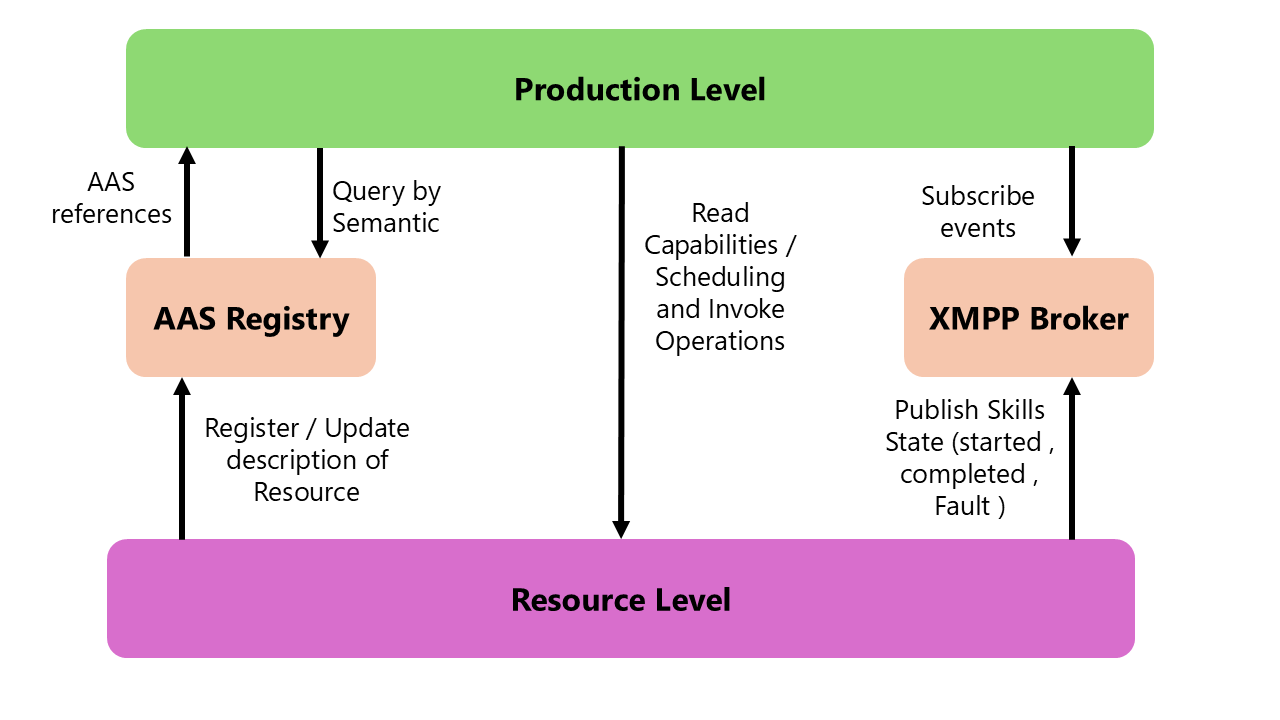
\includegraphics[width=12cm]{Images/system_levels.png}
    \caption{Two-Level System Architecture}
    \label{fig:system_levels}
\end{figure}

\textbf{Product Level.} The product level contains the ProductionAAS, which is responsible for managing production orders and coordinating the allocation of tasks to available resources. When a drilling order is received, the ProductionAAS queries the AAS Registry to discover available resources, retrieves their capabilities, and initiates negotiations to select the most suitable resource for the task. The ProductionAAS subscribes to events published by ResourceAAS instances to monitor execution progress and react to status changes.

\textbf{Resource Level.} The resource level contains one or more ResourceAAS instances, each representing a physical drill machine. ResourceAAS components register themselves with the AAS Registry upon initialization, making their capabilities discoverable. During operation, ResourceAAS instances publish status events (started, completed, fault) to the XMPP Broker, enabling real-time monitoring by the ProductionAAS and other system components. When assigned a production task, the ResourceAAS agent autonomously executes the drilling operation by invoking standardized \ac{AAS} Operations on the physical asset.

\subsection{System Components}
The complete system comprises five main components that work together to realize \ac{Type3AAS} functionality. Figure~\ref{fig:system_architecture} illustrates the overall system architecture and the relationships between components.


\begin{figure}[p]
    \centering
    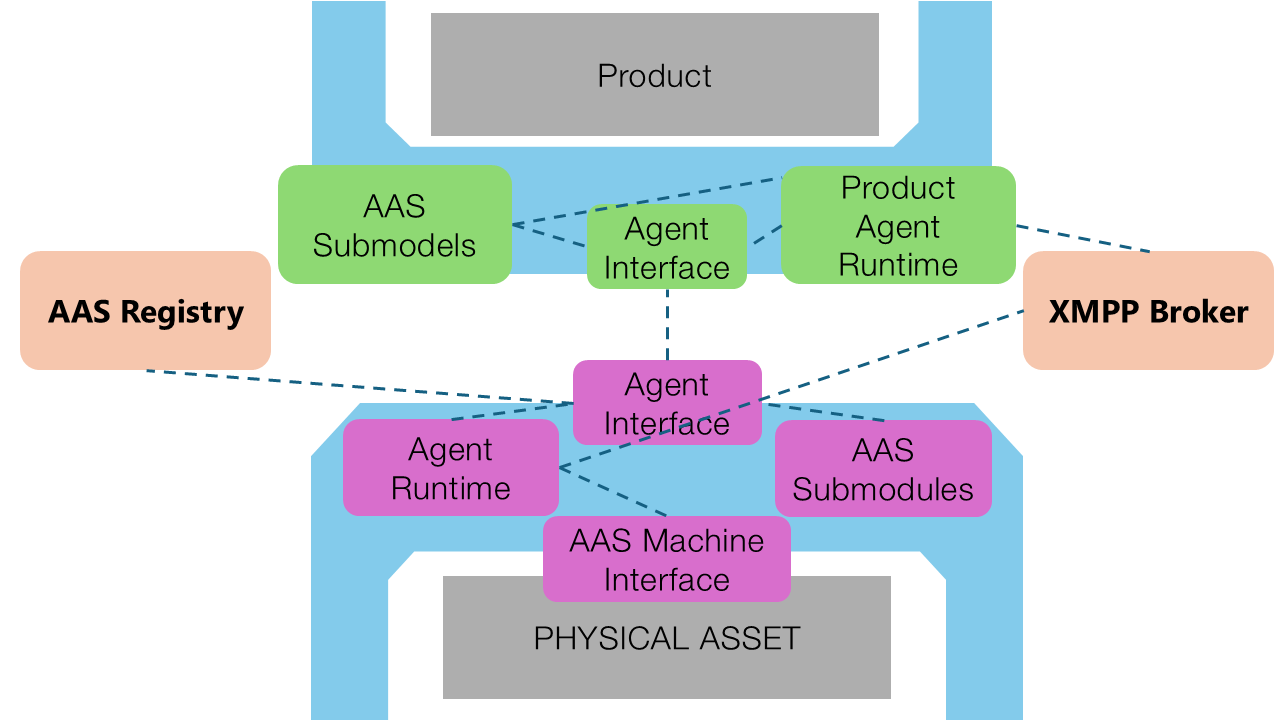
\includegraphics[width=14cm]{Images/system_architecture.png}
    \caption{SmartDrillSystem Architecture Overview}
    \label{fig:system_architecture}
\end{figure}

\textbf{ProductionAAS.} The ProductionAAS serves as the coordination hub for production orders. It combines standardized \ac{AAS} submodels with a \ac{BDI} agent runtime that provides autonomous decision-making capabilities. The ProductionAAS contains submodels for identification, process planning, service cataloging, interface endpoints, and execution tracking. Its agent component implements orchestration logic for task decomposition and negotiation protocols for resource selection. Communication with other components occurs through the Agent Interface, which translates between \ac{AAS} data structures and agent beliefs.

\textbf{ResourceAAS.} Each ResourceAAS represents a digital twin of a physical drill machine, integrating \ac{AAS} standardization with autonomous agent behavior. The ResourceAAS contains submodels describing the asset's operational state, knowledge constraints, capabilities, and interaction parameters. A \ac{BDI} agent runtime provides goal-directed behavior, enabling the resource to autonomously respond to production requests, participate in negotiations, and execute assigned tasks. The AAS Machine Interface connects the digital representation to the physical asset, enabling bidirectional data exchange and operation invocation.

\textbf{AAS Registry.} The AAS Registry provides a centralized discovery service compliant with the \ac{AAS} specification. Upon initialization, each ResourceAAS registers its identification information, endpoint addresses, and capability descriptions with the registry. The ProductionAAS queries the registry to discover available resources that match required capabilities. This decoupled discovery mechanism enables dynamic system reconfiguration without hardcoded dependencies between components.

\textbf{XMPP Broker.} The XMPP Broker implements the event-driven communication infrastructure using the \ac{XMPP} protocol. This choice aligns with the SPADE framework used for agent implementation, which natively supports \ac{XMPP} for agent communication. The broker enables publish-subscribe messaging patterns where ResourceAAS instances publish status events (skill started, completed, or failed) and the ProductionAAS subscribes to receive these updates. This asynchronous communication model supports reactive agent behavior and real-time monitoring.

\textbf{Physical Assets.} The physical drill machines represent the actual manufacturing resources controlled by the system. Each asset connects to its corresponding ResourceAAS through a machine interface that abstracts the underlying communication protocol (such as OPC UA or proprietary interfaces). The ResourceAAS reads sensor data and operational status from the asset and invokes operations to execute drilling tasks.
\subsection{Component Interactions}
Figure~\ref{fig:component_interactions} illustrates the interaction patterns between system components during typical operation.


\begin{figure}[p]
    \centering
    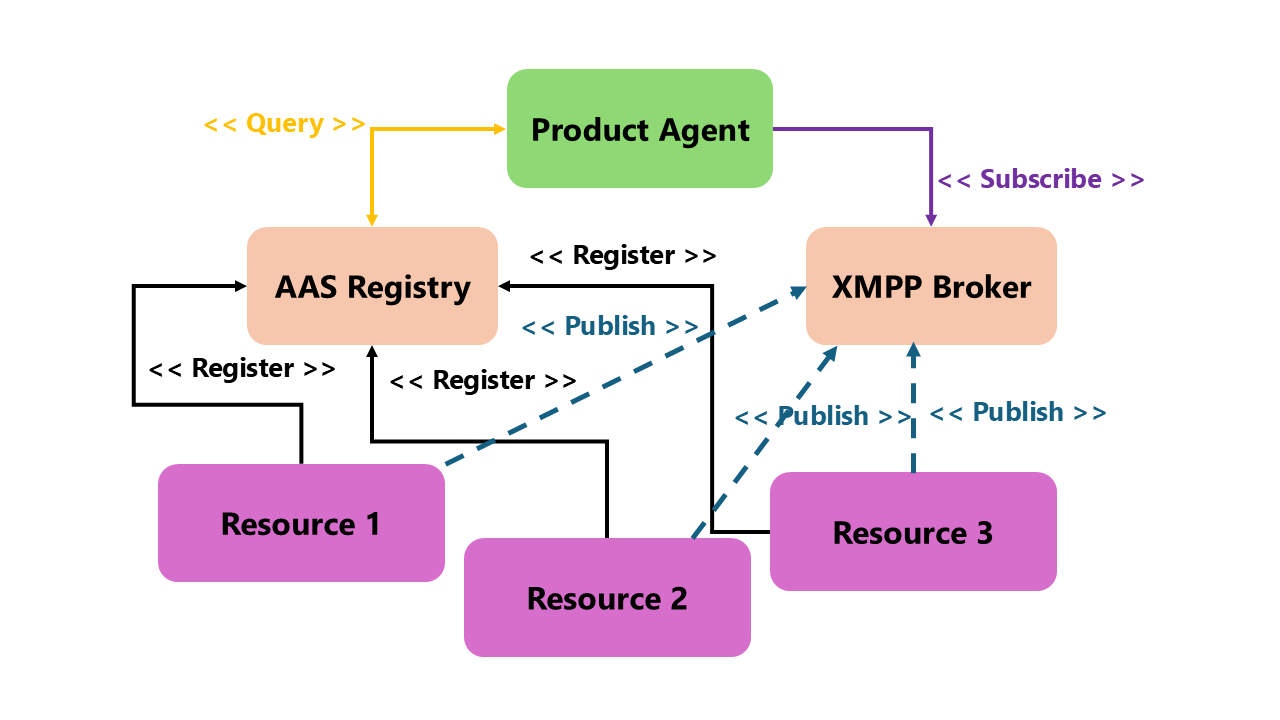
\includegraphics[width=12cm]{Images/component_interactions.png}
    \caption{Component Interaction Patterns}
    \label{fig:component_interactions}
\end{figure}

The system employs four primary interaction patterns:

\textbf{Registration.} During system startup, each ResourceAAS registers itself with the AAS Registry and the XMPP Broker. Registration with the registry enables discovery by the ProductionAAS, while registration with the broker enables event publication and subscription.

\textbf{Discovery.} When the ProductionAAS receives a production order, it queries the AAS Registry to retrieve references to all registered ResourceAAS instances. The registry returns the endpoint addresses and capability descriptions needed to initiate direct communication with resources.

\textbf{Direct Communication.} The ProductionAAS communicates directly with ResourceAAS instances for operations requiring request-response patterns, such as reading capabilities, scheduling information, and invoking operations. This communication uses the standardized \ac{AAS} REST API, ensuring interoperability with the \ac{AAS} specification.

\textbf{Event-Based Communication.} ResourceAAS instances publish status events to the XMPP Broker, and the ProductionAAS subscribes to receive these events. This pattern supports asynchronous notification of state changes without requiring polling, enabling efficient real-time monitoring of distributed resources.


\subsection{Bidirectional AAS Integration}

A key contribution of this design is the bidirectional integration between \ac{BDI} agents and the \ac{AAS} standard. Unlike existing approaches that use \ac{AAS} primarily as a passive data source, this architecture enables agents to both read information from submodels and execute actions through standardized Operations.

\textbf{Beliefs from Submodels.} Agent beliefs are derived from \ac{AAS} submodel data. The Operational State Submodel provides current asset status, the Knowledge Submodel provides constraints and environmental conditions, and the Capability Submodel provides information about available skills. The Agent Interface continuously synchronizes submodel data with the agent's belief base, ensuring that agent decisions reflect the current system state.

\textbf{Intentions through Operations.} Agent intentions are executed through \ac{AAS} Operations defined in the submodels. When an agent commits to executing a drilling task, it invokes the corresponding Operation on the physical asset through the standardized \ac{AAS} API. This approach leverages the Operation element defined in the \ac{AAS} specification, which supports both synchronous and asynchronous invocation patterns.

This bidirectional integration ensures that the autonomous behavior provided by the \ac{BDI} architecture operates within the standardized framework defined by the \ac{AAS} specification, addressing the interoperability requirements identified in Chapter~\ref{ch:literature}.

\subsection{Mapping to RAMI4.0}
\label{subsec:rami40_mapping}

The proposed Type 3 \ac{AAS} architecture can be positioned within the \ac{RAMI4.0} reference model introduced in Chapter~\ref{ch:introduction}. Figure~\ref{fig:RAMI4.0} presents the three-dimensional RAMI4.0 structure consisting of Hierarchy Levels, Life Cycle \& Value Stream, and Layers. This subsection maps the system components to each axis.

\subsubsection{Hierarchy Levels Axis}

The system operates across multiple hierarchy levels as defined by IEC 62264:

\begin{table}[ht]
\centering
\caption{System Components Mapped to RAMI4.0 Hierarchy Levels}
\label{tab:rami_hierarchy}
\begin{tabular}{p{0.20\textwidth}p{0.25\textwidth}p{0.45\textwidth}}
\toprule
\rowcolor{headerblue}
\textcolor{white}{Hierarchy Level} & \textcolor{white}{Component} & \textcolor{white}{Role} \\
\midrule
Work Centers & Production Agent & Coordinates production orders, orchestrates resources \\
\rowcolor{lightgray}
Station & Resource Agent & Manages individual drill machine operations \\
Field Device & Simulators / PLCs & Executes physical operations (drill, move) \\
\bottomrule
\end{tabular}
\end{table}

The Production Agent operates at the \textit{Work Centers} level, receiving production orders and coordinating their execution across available resources. Resource Agents operate at the \textit{Station} level, each representing a single manufacturing resource (drill machine). The simulators (or physical PLCs in a production deployment) represent the \textit{Field Device} level, executing the actual machining operations.

\subsubsection{Life Cycle \& Value Stream Axis}

The RAMI4.0 life cycle axis distinguishes between \textit{Type} (design-time definitions) and \textit{Instance} (runtime representations):

\begin{table}[ht]
\centering
\caption{System Elements Mapped to RAMI4.0 Life Cycle Phases}
\label{tab:rami_lifecycle}
\begin{tabular}{p{0.15\textwidth}p{0.35\textwidth}p{0.40\textwidth}}
\toprule
\rowcolor{headerblue}
\textcolor{white}{Phase} & \textcolor{white}{Type (Design)} & \textcolor{white}{Instance (Runtime)} \\
\midrule
Development & Submodel templates, Capability definitions & -- \\
\rowcolor{lightgray}
Maintenance & Process Plan structure, Knowledge constraints & -- \\
Production & -- & AAS instances, Agent beliefs, Execution state \\
\bottomrule
\end{tabular}
\end{table}

The submodel structures (Capability, Knowledge, Process Plan) represent \textit{Type} information reusable templates that define what a resource can do and how processes are structured. At runtime, these become \textit{Instance} data: concrete AAS instances with actual parameter values, agent beliefs reflecting current state, and execution tracking data that changes during operation.

\subsubsection{Layer Axis}

The six RAMI4.0 layers describe different aspects of an \ac{I4.0} component. Table~\ref{tab:rami_layers} maps the system implementation to each layer:

\begin{table}[ht]
\centering
\caption{System Implementation Mapped to RAMI4.0 Layers}
\label{tab:rami_layers}
\begin{tabular}{p{0.18\textwidth}p{0.72\textwidth}}
\toprule
\rowcolor{headerblue}
\textcolor{white}{Layer} & \textcolor{white}{Implementation} \\
\midrule
Business & Production orders (User Requests) triggering manufacturing processes \\
\rowcolor{lightgray}
Functional & BDI agent logic: goal-directed reasoning, plan execution, CNP negotiation \\
Information & AAS submodels: Capability, Knowledge, Process Plan, Execution Tracking \\
\rowcolor{lightgray}
Communication & XMPP PubSub (agent messaging), REST API (AAS access), HTTP (skill invocation) \\
Integration & ResourceAASClient, invocationDelegation pattern, BaSyx SDK \\
\rowcolor{lightgray}
Asset & Drill machine simulators (proof-of-concept) / Physical PLCs (production) \\
\bottomrule
\end{tabular}
\end{table}

\textbf{Business Layer.} Production orders represent business-level requests that initiate the manufacturing process. The User Request message defines what capability is needed and when.

\textbf{Functional Layer.} The \ac{BDI} agent architecture provides the functional logic. Agents reason about their beliefs (from submodels), form desires (respond to CFP, execute skills), and commit to intentions (negotiate, invoke operations). This layer realizes the ``proactive'' behavior that distinguishes Type 3 from Type 1/2 \ac{AAS}.

\textbf{Information Layer.} The \ac{AAS} submodels provide the standardized information model. All data exchanged between components conforms to the \ac{AAS} meta-model, ensuring interoperability with other I4.0-compliant systems.

\textbf{Communication Layer.} Three protocols handle different communication needs: XMPP PubSub for asynchronous agent messaging and event notification, the \ac{AAS} REST API for submodel access, and HTTP for skill invocation via the invocationDelegation pattern.

\textbf{Integration Layer.} The ResourceAASClient and ProductionAASClient classes bridge the gap between the \ac{AAS} server and the agent runtime. The invocationDelegation qualifier pattern connects \ac{AAS} Operations to external execution endpoints.

\textbf{Asset Layer.} The physical drill machines (represented by simulators in the proof-of-concept) form the asset layer. These execute the actual manufacturing operations when invoked through the integration layer.

\subsubsection{Type 3 AAS in the RAMI4.0 Context}

The key contribution of this work within the RAMI4.0 framework is the enhancement of the \textit{Functional Layer}. While Type 1 and Type 2 \ac{AAS} implementations primarily address the Information, Communication, and Integration layers, the Type 3 \ac{AAS} adds autonomous decision-making capabilities at the Functional Layer through \ac{BDI} agent integration.

This positions the Type 3 \ac{AAS} as an enabler for the RAMI4.0 vision of intelligent, self-organizing production systems where I4.0 components can autonomously coordinate without centralized control.
\section{Resource Agent Concept}
\label{sec:resource_agent}

The ResourceAAS represents the core component for integrating autonomous agent behavior with standardized \ac{AAS} representations of manufacturing resources. This section presents the conceptual design of the ResourceAAS, describing its overall architecture, submodel structure, agent core, and the mechanisms that enable bidirectional integration between the \ac{BDI} agent and the \ac{AAS}.

\subsection{Resource Agent Overview}
\label{subsec:resource_overview}

The ResourceAAS combines three main architectural elements: the \ac{AAS} structure providing standardized data representation, the \ac{BDI} agent core enabling autonomous behavior, and the interfaces connecting these components to each other and to external systems. Figure~\ref{fig:resource_components} illustrates the high-level component structure of the ResourceAAS.

% Include diagram from slide 5
\begin{figure}[p]
    \centering
    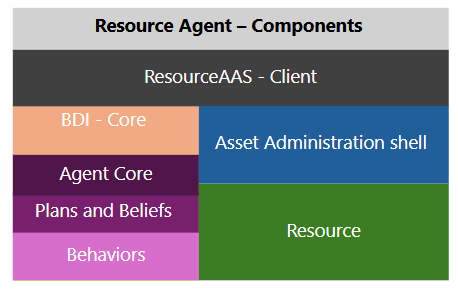
\includegraphics[width=10cm]{Images/resource_components.png}
    \caption{Resource Agent Component Structure}
    \label{fig:resource_components}
\end{figure}

\textbf{Asset Administration Shell.} The \ac{AAS} component provides the standardized digital representation of the drill machine using the Eclipse BaSyx Python SDK. It contains the shell information (identification, asset kind, global asset ID) and a collection of submodels that describe different aspects of the resource. The \ac{AAS} is deployed to a BaSyx AAS Environment server, exposing a REST API that enables external access to submodel data and operation invocation, compliant with the \ac{AAS} API specification defined in Part 2 of the standard.

\textbf{BDI Core.} The \ac{BDI} core implements the agent's autonomous behavior using the SPADE framework combined with the spade\_bdi extension. SPADE (Smart Python Agent Development Environment) provides asynchronous agent communication over \ac{XMPP}, while spade\_bdi adds AgentSpeak-based \ac{BDI} reasoning capabilities. The agent maintains beliefs derived from submodel data, processes desires triggered by external events (such as Call-For-Proposals), and executes intentions through SPADE behaviors. Agent plans are defined in AgentSpeak Language (ASL) files that specify reactive rules for handling events and achieving goals.

\textbf{AAS-Agent Interface (ResourceAASClient).} The ResourceAASClient serves as the translation layer between the \ac{AAS} REST API and the agent's internal representation. This component implements an asynchronous HTTP client using aiohttp that communicates with the BaSyx server via GET and POST requests. It provides repository classes for reading submodel elements (SubmodelElementRepositoryGetters), updating values (SubmodelElementRepositoryUpdate), and invoking operations. The interface translates \ac{AAS} data structures into Python dictionaries that can be converted to agent beliefs.

\textbf{Operation Invokers.} The physical asset operations are exposed through FastAPI-based HTTP endpoints that implement the invocationDelegation pattern specified in the \ac{AAS} Operation qualifiers. When the BaSyx server receives an operation invocation request, it delegates the call to the corresponding invoker endpoint (e.g., \texttt{/drill\_invocation\_1}), which executes the operation on the physical asset or simulator and returns the result.

Figure~\ref{fig:resource_internal} illustrates the internal connections and data flows within the ResourceAAS architecture.

% Include diagram from slide 6 or 16
\begin{figure}[p]
    \centering
    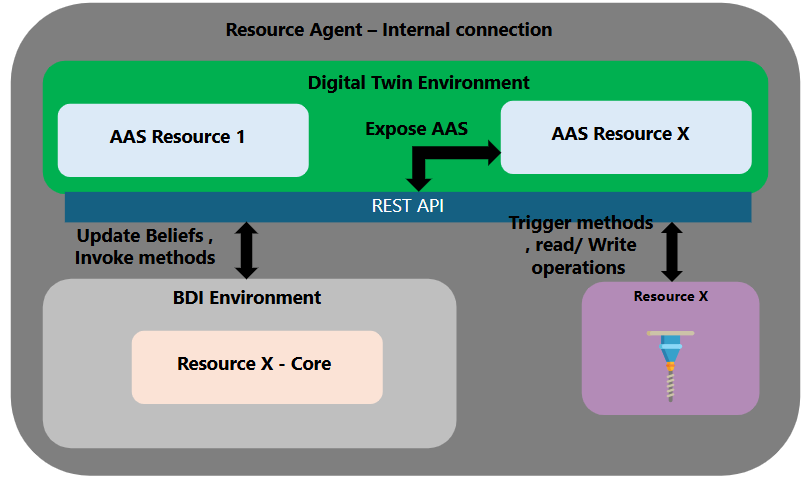
\includegraphics[width=12cm]{Images/resource_internal.png}
    \caption{Resource Agent Internal Architecture}
    \label{fig:resource_internal}
\end{figure}

The architecture supports three primary data flows:

\textbf{Belief Acquisition.} During agent initialization, the AgentInitializationbehavior reads submodel data via the ResourceAASClient and populates the agent's belief base. Beliefs include: \texttt{current\_state} from the Operational State Submodel, \texttt{supported\_skills} from the Capabilities Submodel, \texttt{skills\_constraints} from the Knowledge Submodel, and \texttt{free\_time\_slots} / \texttt{booked\_time\_slots} from the Operational State time slot collection.

\textbf{Event Processing.} When the agent receives a Call-For-Proposal (CFP) from the ProductionAAS via \ac{XMPP} publish-subscribe, the CFPProcessingbehavior validates the request against current beliefs. It checks whether the resource state allows execution, whether the requested skill is supported, and whether input parameters fall within the constraints defined in the Knowledge Submodel.

\textbf{Operation Execution.} When the agent commits to executing a task, the corresponding invoker behavior (e.g., DrillInvokerbehavior) retrieves input parameters from beliefs, calls the operation through the ResourceAASClient, and updates beliefs with the result. The operation invocation follows the \ac{AAS} standard, passing through the BaSyx server to the delegated FastAPI endpoint.

\subsection{Resource Agent Submodels}
\label{subsec:resource_submodels}

The ResourceAAS contains four submodels that provide the standardized data structures supporting agent operation. These submodels are implemented using the Eclipse BaSyx Python SDK and are designed to map directly to the \ac{BDI} components. The following subsections describe each submodel based on the actual implementation.


\subsubsection{Operational State Submodel}

The Operational State Submodel captures the current runtime status and scheduling information of the resource. It provides the primary source for agent beliefs about the asset's availability and current condition. Figure~\ref{fig:sm_operational_state} shows the structure of this submodel.

\begin{figure}[p]
    \centering
    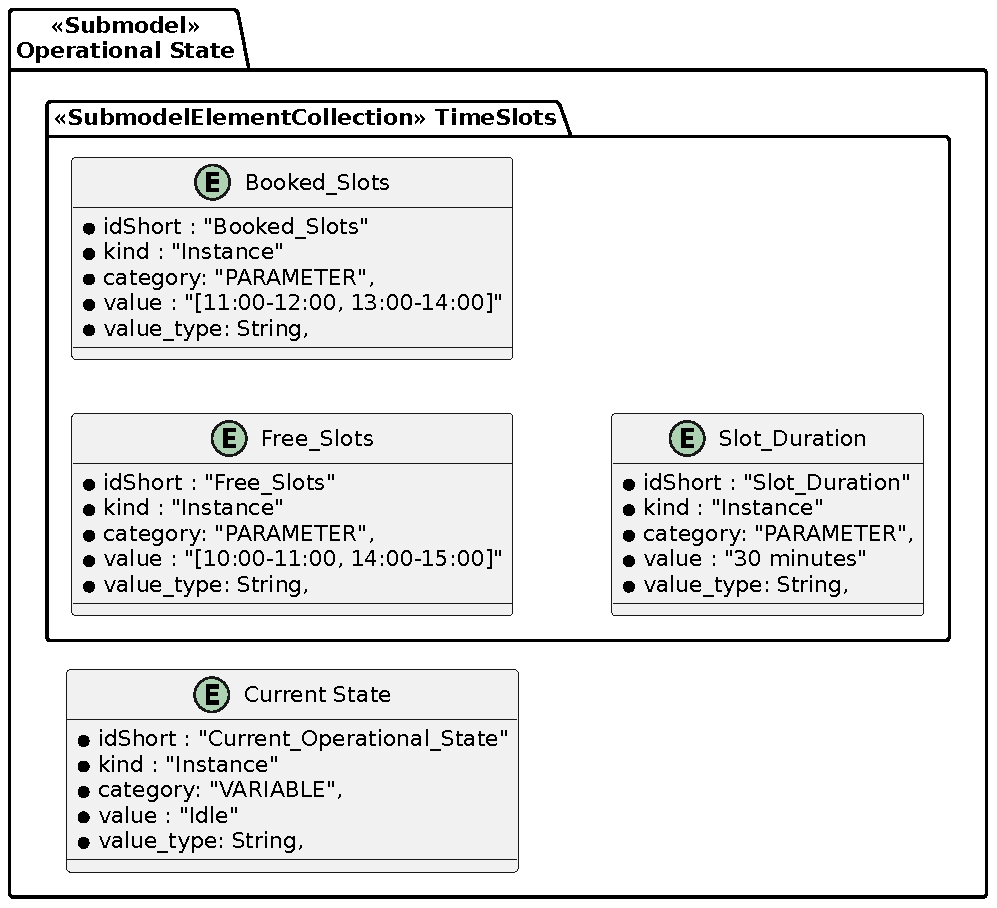
\includegraphics[width=0.85\textwidth]{Images/sm_operational_state.pdf}
    \caption{Operational State Submodel Structure}
    \label{fig:sm_operational_state}
\end{figure}

\textbf{Current\_Operational\_State.} This Property element tracks the real-time operational status of the drill machine. The value contains the current state as a string (``Idle'', ``Running'', ``Error'', or ``Done''), with the category set to ``VARIABLE'' indicating runtime mutability. During CFP processing, the agent checks this belief to ensure the resource is in an allowed state (``Idle'' or ``Free'') before accepting new tasks.

\textbf{TimeSlots\_Operational\_Data.} This SubmodelElementCollection manages the resource's scheduling information through three properties:
\begin{itemize}
    \item \texttt{Free\_Slots}: JSON-encoded list of available time slots (e.g., ``08:00'', ``08:30'', ``09:00'')
    \item \texttt{Booked\_Slots}: JSON-encoded list of already allocated time slots
    \item \texttt{Slot\_Duration}: Integer value representing the duration of each slot in minutes
\end{itemize}
The TimeSlotDataType class manages slot allocation and release, ensuring that negotiation decisions are based on actual availability.

\subsubsection{Knowledge Submodel}

The Knowledge Submodel contains constraint information that defines the operational boundaries of the resource. This information is used during CFP validation to determine whether requested parameters are feasible. Figure~\ref{fig:sm_knowledge} shows the structure of this submodel.
\subsubsection{Knowledge Submodel}

The Knowledge Submodel contains constraint information that defines the operational boundaries of the resource. This information is used during CFP validation to determine whether requested parameters are feasible. Figure~\ref{fig:sm_knowledge} shows the structure of this submodel.

\begin{figure}[p]
    \centering
    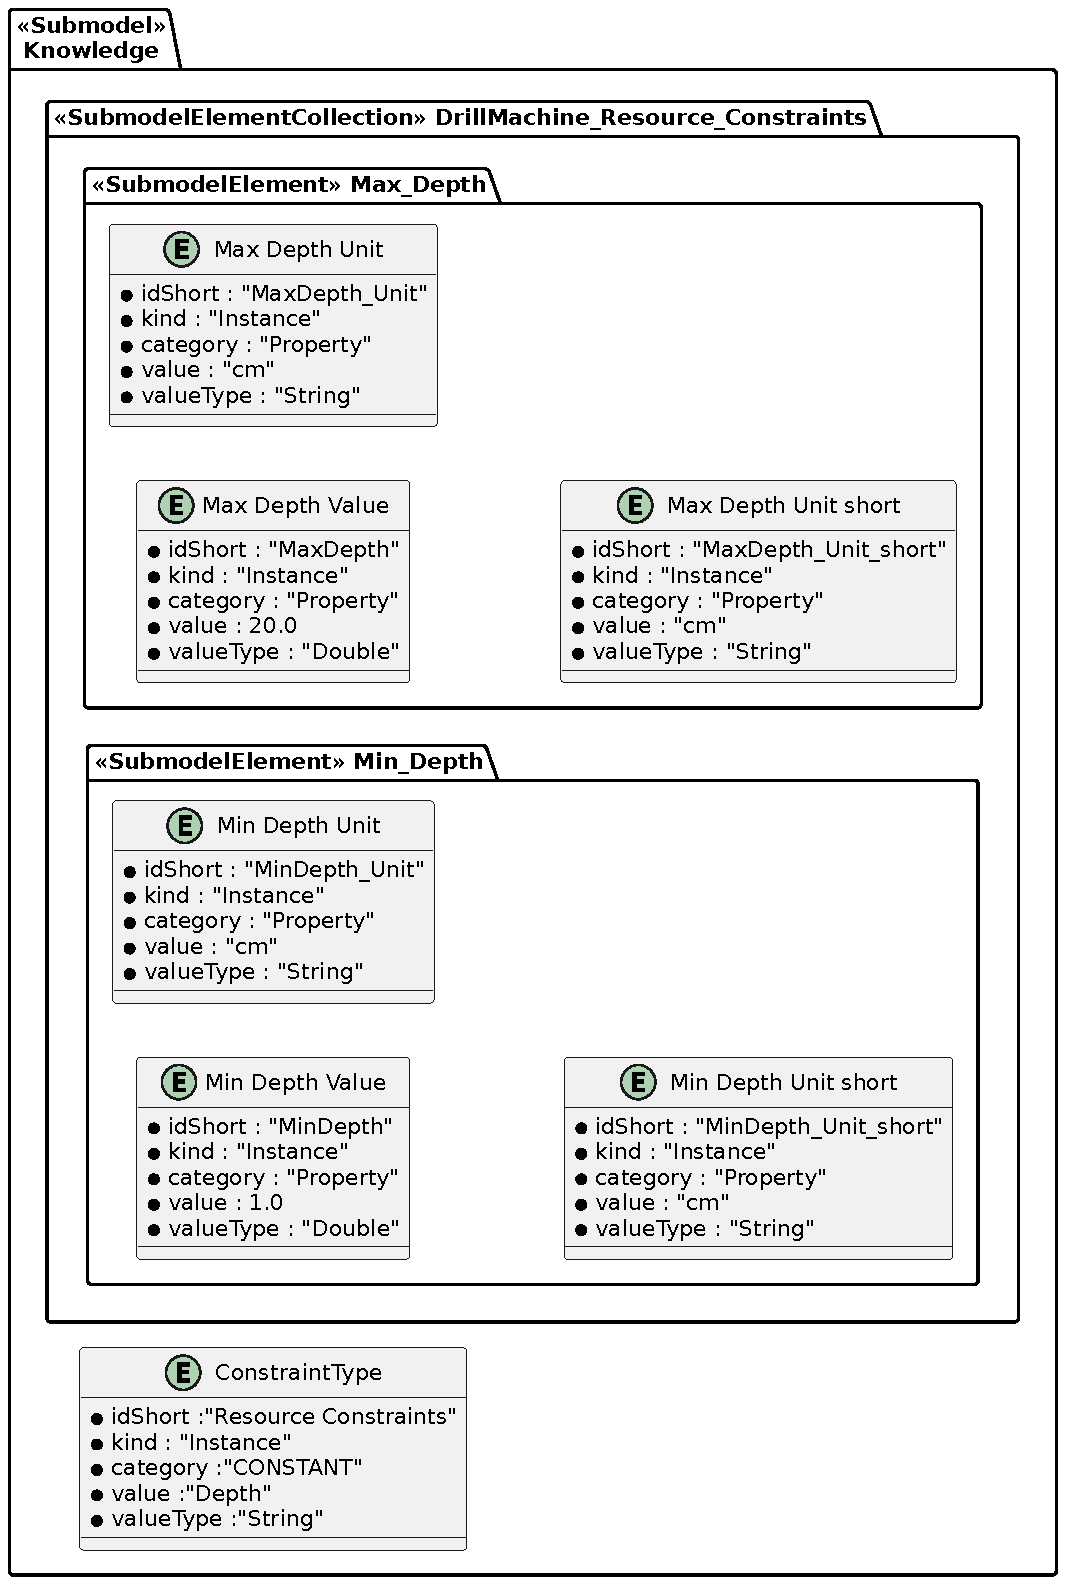
\includegraphics[width=0.85\textwidth]{Images/sm_knowledge.pdf}
    \caption{Knowledge Submodel Structure}
    \label{fig:sm_knowledge}
\end{figure}

\textbf{Resource\_Constraints.} This SubmodelElementCollection contains nested collections for each constraint type:
\begin{itemize}
    \item \texttt{MaxDepth}: Collection with MaxDepthValue (Double, e.g., 20.0), MaxDepthUnit (``centimeters''), and MaxDepthUnitShort (``cm'')
    \item \texttt{MinDepth}: Collection with MinDepthValue (Double, e.g., 1.0) and corresponding unit properties
    \item \texttt{ConstraintType}: Property indicating the parameter being constrained (``Depth'')
\end{itemize}

During CFP processing, the agent retrieves the constraint type and min/max values, then validates that the requested input parameter falls within the allowed range. If validation fails, a \texttt{CONSTRAINT\_VIOLATION} is added to the negotiation response.

\subsubsection{Capability Submodel}

The Capability Submodel describes the skills and operations that the resource can perform. This submodel directly relates to agent capabilities and contains the Operation elements that enable bidirectional integration. Figure~\ref{fig:sm_capability} shows the structure of this submodel.

\begin{figure}[p]
    \centering
    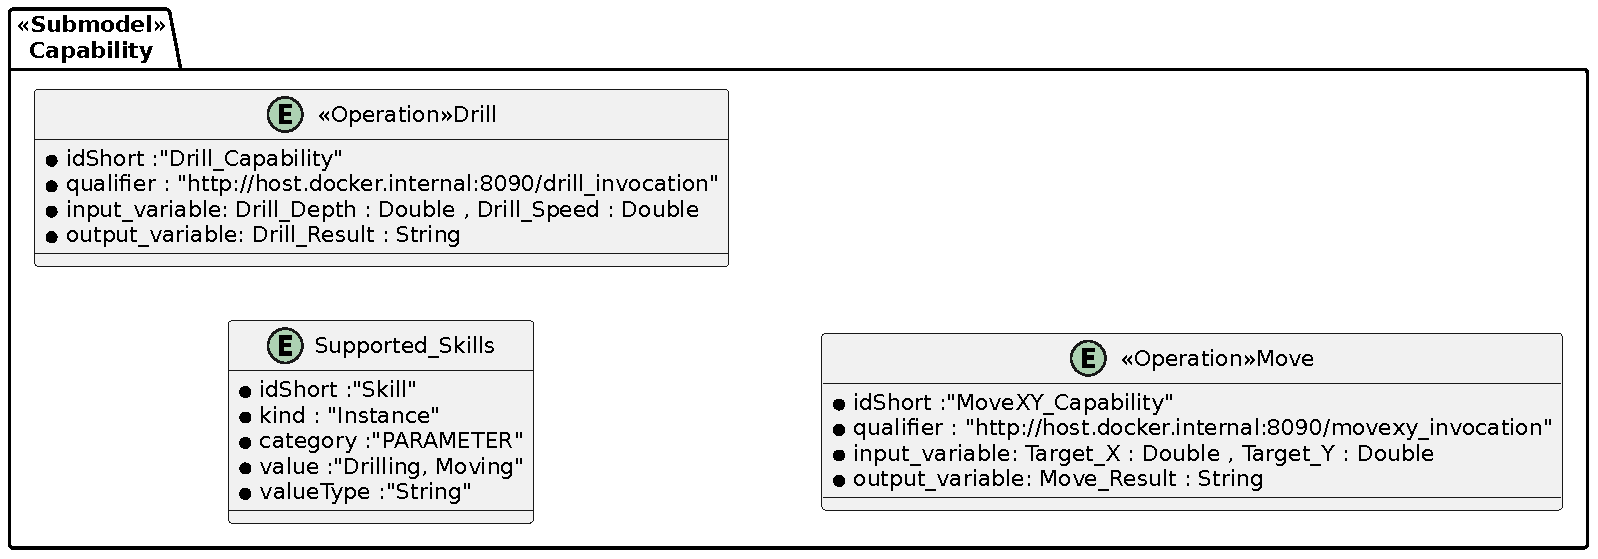
\includegraphics[width=0.95\textwidth]{Images/sm_capability.pdf}
    \caption{Capability Submodel Structure}
    \label{fig:sm_capability}
\end{figure}

\textbf{Supported\_Skills.} This Property lists the capabilities supported by the resource as a comma-separated string (e.g., ``drill\_capability,movexy\_capability''). The ProductionAAS uses this information during resource discovery to filter resources that can fulfill requested operations.

\textbf{Drill\_Capability.} This Operation element defines the drilling capability with:
\begin{itemize}
    \item \texttt{invocationDelegation} qualifier: URL of the FastAPI endpoint
    \item Input variables: Drill\_Depth (Double) and Drill\_Speed (Double)
    \item Output variable: Drill\_Result (String)
\end{itemize}

\textbf{MoveXY\_Capability.} This Operation element defines the positioning capability with:
\begin{itemize}
    \item \texttt{invocationDelegation} qualifier: URL of the movement endpoint
    \item Input variables: Target\_X (Double) and Target\_Y (Double)
    \item Output variable: Move\_Result (String)
\end{itemize}

The invocationDelegation pattern enables the BaSyx server to forward operation requests to external services, supporting integration with physical assets or simulators without modifying the \ac{AAS} infrastructure.

\subsubsection{Interaction and Scheduling Submodel}

The Interaction and Scheduling Submodel provides the communication endpoints through which external systems can interact with the ResourceAAS. Figure~\ref{fig:sm_interaction} shows the structure of this submodel.

\begin{figure}[p]
    \centering
    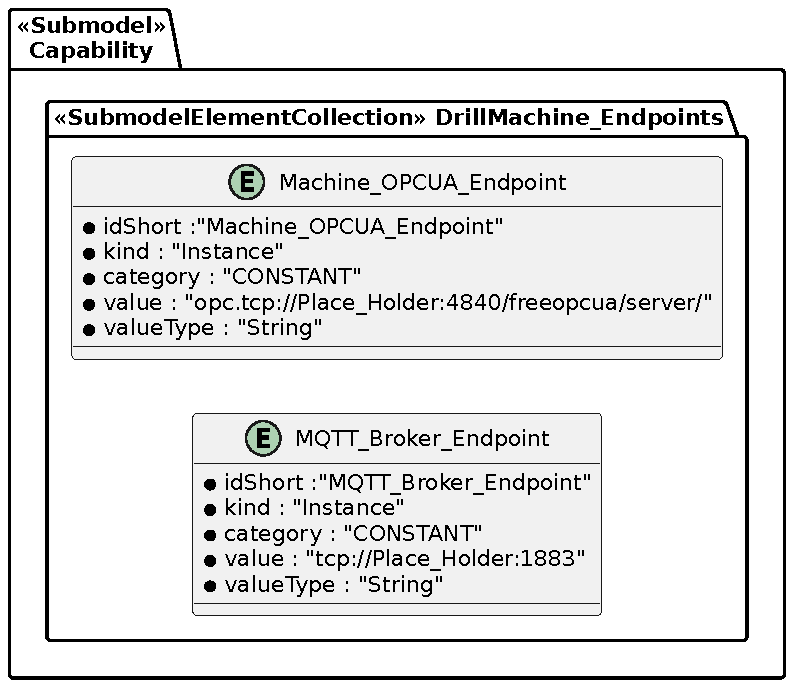
\includegraphics[width=0.6\textwidth]{Images/sm_interaction.pdf}
    \caption{Interaction and Scheduling Submodel Structure}
    \label{fig:sm_interaction}
\end{figure}

\textbf{Endpoints.} This SubmodelElementCollection contains properties for different communication protocols:
\begin{itemize}
    \item \texttt{Machine\_OPCUA\_Endpoint}: OPC UA server address for direct asset communication (placeholder for future integration)
    \item \texttt{MQTT\_Broker\_Endpoint}: MQTT broker address for event-based communication
\end{itemize}

The ProductionAAS retrieves these endpoints during the discovery phase to establish appropriate communication channels for negotiation and task assignment.


\subsection{BDI-Submodel Integration}
\label{sec:bdi_submodel_integration}

This section explicitly describes how the \ac{BDI} architecture manifests in the Type 3 \ac{AAS} implementation. The title of this thesis references \ac{BDI} agents, and this section clarifies how Beliefs, Desires, and Intentions are concretely realized through the \ac{AAS} submodels and AgentSpeak plans.
\subsubsection{Conceptual Mapping}

The \ac{BDI} model defines three mental attitudes that govern agent behavior:
\begin{itemize}
    \item \textbf{Beliefs}: The agent's knowledge about itself, other agents, and the environment
    \item \textbf{Desires}: The agent's objectives or goals it wishes to achieve
    \item \textbf{Intentions}: The agent's committed plans for achieving its goals
\end{itemize}
In the Type 3 \ac{AAS} architecture, these mental attitudes are distributed between the \ac{AAS} submodels (persistent, shared state) and the AgentSpeak plans (reactive behavior). Table~\ref{tab:bdi_mapping} provides the concrete mapping.

\begin{table}[p]
\centering
\caption{BDI to AAS-Agent Mapping}
\label{tab:bdi_mapping}
\begin{tabular}{p{0.12\textwidth}p{0.28\textwidth}p{0.48\textwidth}}
\toprule
\rowcolor{headerblue}
\textcolor{white}{BDI Element} & \textcolor{white}{AAS/Agent Component} & \textcolor{white}{Concrete Example} \\
\midrule
Beliefs & Operational State Submodel & \texttt{current\_state}, \texttt{free\_time\_slots} \\
        & Knowledge Submodel & \texttt{skills\_constraints}, \texttt{skills\_constraints\_types} \\
        & Capability Submodel & \texttt{supported\_skills} \\
        & Runtime Beliefs & \texttt{is\_cfp\_received}, \texttt{cfp\_skill}, \texttt{cfp\_at\_time} \\
\midrule
\rowcolor{lightgray}
Desires & AgentSpeak Goals & \texttt{!setup} (initialization goal) \\
\rowcolor{lightgray}
        & Event-triggered Goals & Respond to CFP, execute skills \\
\rowcolor{lightgray}
        & Process Plan & Reach \texttt{Exit\_Point} from \texttt{Entry\_Point} \\
\midrule
Intentions & AgentSpeak Plans & Plans triggered by belief additions \\
           & Custom Actions & \texttt{.initialize\_agent}, \texttt{.process\_cfp}, \texttt{.drill} \\
           & SPADE behaviors & \texttt{DrillInvokerbehavior}, \texttt{MoveXYInvokerbehavior} \\
\bottomrule
\end{tabular}
\end{table}

\subsubsection{Beliefs: AAS Submodels as Knowledge Base}

The agent's beliefs are loaded from \ac{AAS} submodels during initialization via the \texttt{AgentInitializationbehavior}. This behavior reads submodel data and converts it to agent beliefs:

\begin{lstlisting}[language=Python, caption={Belief Loading from AAS Submodels}, label={lst:belief_loading}]
class AgentInitializationbehavior(OneShotbehavior):
    async def run(self):
        # Load beliefs from AAS submodels concurrently
        current_state, skills, constraints, ... = await asyncio.gather(
            self.agent.resource_client.getvalue_Current_State(),
            self.agent.resource_client.getvalue_Supported_Skills(),
            self.agent.resource_client.getvalue_MaxMinDepth(),
            self.agent.resource_client.getvalue_Free_Slots(),
            ...
        )
        # Set beliefs in BDI agent
        self.agent.bdi.set_belief("current_state", current_state)
        self.agent.bdi.set_belief("supported_skills", skills)
        self.agent.bdi.set_belief("skills_constraints", constraints)
        self.agent.bdi.set_belief("free_time_slots", free_time_slots)
\end{lstlisting}
Table~\ref{tab:belief_sources} shows the mapping between \ac{AAS} submodel elements and agent beliefs:

\begin{table}[p]
\centering
\caption{AAS Submodel Elements to Agent Beliefs}
\label{tab:belief_sources}
\begin{tabular}{lll}
\toprule
\rowcolor{headerblue}
\textcolor{white}{Submodel} & \textcolor{white}{Element} & \textcolor{white}{Belief Predicate} \\
\midrule
Operational State & Current\_State & \texttt{current\_state(State)} \\
Operational State & Free\_Slots & \texttt{free\_time\_slots(Slots)} \\
Operational State & Booked\_Slots & \texttt{booked\_time\_slots(Slots)} \\
\rowcolor{lightgray}
Capability & Supported\_Skills & \texttt{supported\_skills(Skills)} \\
\rowcolor{lightgray}
Knowledge & Constraints & \texttt{skills\_constraints(Values)} \\
Knowledge & Constraints\_Type & \texttt{skills\_constraints\_types(Types)} \\
\bottomrule
\end{tabular}
\end{table}
\textbf{Runtime Beliefs.} In addition to persistent beliefs from submodels, the agent maintains runtime beliefs that change during execution:
\begin{itemize}
    \item \texttt{is\_cfp\_received(true/false)}: Set when a CFP message arrives
    \item \texttt{cfp\_skill(Skill)}: The requested capability from the CFP
    \item \texttt{cfp\_at\_time(TimeSlot)}: The requested time slot
    \item \texttt{current\_operation(drill/movexy)}: Tracks which operation is executing
    \item \texttt{drill\_completed(true)}, \texttt{move\_xy\_completed(true)}: Operation completion flags
\end{itemize}

\subsubsection{Desires: Goals in AgentSpeak}

Desires represent what the agent wants to achieve. In the implementation, desires are expressed through AgentSpeak achievement goals and event-triggered responses:

\textbf{Initialization Goal.} The agent starts with an explicit goal:
\begin{lstlisting}[language=Prolog, caption={Initial Goal in AgentSpeak}, label={lst:initial_goal}]
!setup.

+!setup <-
  .print("Agent started : Drilling Machine 1");
  .initialize_agent;
  .check_request.
\end{lstlisting}

\textbf{Event-Triggered Desires.} Most desires emerge from belief changes rather than explicit goal statements. When a belief is added, it triggers a plan that implicitly represents a desire:

\begin{lstlisting}[language=Prolog, caption={Desire: Respond to CFP}, label={lst:cfp_desire}]
// Desire: When CFP received, respond appropriately
+is_cfp_received(true) <-
  -is_cfp_received(true);
  .print("EVENT: CFP received, processing Time slots");
  .process_time_slots;
  .process_cfp.
\end{lstlisting}

\begin{lstlisting}[language=Prolog, caption={Desire: Execute Skills}, label={lst:execute_desire}]
// Desire: When selected, execute the requested skills
+excute_skills(drill_capability) <-
  -excute_skills(drill_capability);
  +current_operation(drill);
  .print("Drilling - starting move_xy");
  .move_xy.
\end{lstlisting}

\subsubsection{Intentions: Committed Plans and Actions}
Intentions are the plans the agent commits to execute. They bridge desires to concrete actions through custom actions and SPADE behaviors:

\textbf{Custom Actions.} The \texttt{ResourceAgent} class registers custom actions that map AgentSpeak action calls to SPADE behaviors:

\begin{lstlisting}[language=Python, caption={Custom Action Registration}, label={lst:custom_actions}]
def add_custom_actions(self, actions):
    @actions.add(".initialize_agent", 0)
    def _initialize_agent(agent, term, intention):
        agent_init_behavior = AgentInitializationbehavior()              
        self.add_behavior(agent_init_behavior)
        yield
        
    @actions.add(".drill", 0)
    def _drill(agent, term, intention):
        drill_behavior = DrillInvokerbehavior()
        self.add_behavior(drill_behavior)
        yield
        
    @actions.add(".move_xy", 0)
    def _move_xy(agent, term, intention):
        move_xy_behavior = MoveXYInvokerbehavior()
        self.add_behavior(move_xy_behavior)
        yield
\end{lstlisting}

\textbf{Intention Execution Flow.} When an AgentSpeak plan executes an action like \texttt{.drill}, the following occurs:
\begin{enumerate}
    \item AgentSpeak interpreter calls the registered custom action
    \item Custom action instantiates the corresponding SPADE behavior
    \item behavior executes asynchronously, invoking the \ac{AAS} Operation
    \item Upon completion, behavior sets a belief (e.g., \texttt{drill\_completed(true)})
    \item Belief change triggers the next plan in the sequence
\end{enumerate}

\textbf{Context-Dependent Plans.} AgentSpeak supports context conditions that select different plans based on current beliefs:

\begin{lstlisting}[language=Prolog, caption={Context-Dependent Intention Selection}, label={lst:context_plans}]
// When move completes during drill operation -> continue to drill
+move_xy_completed(true) : current_operation(drill) <-
  -move_xy_completed(true);
  .print("Move completed, now drilling");
  .drill.

// When move completes during movexy-only operation -> done
+move_xy_completed(true) : current_operation(movexy) <-
  -move_xy_completed(true);
  -current_operation(movexy);
  .print("Move completed, operation done");
  .operation_done.
\end{lstlisting}

This demonstrates how the agent's current beliefs (context) determine which intention is formed, a key characteristic of \ac{BDI} reasoning.
\subsubsection{BDI Reasoning Cycle}
Figure~\ref{fig:bdi_cycle} illustrates how the \ac{BDI} reasoning cycle operates within the Type 3 \ac{AAS}:

\begin{figure}[ht]
\centering
\begin{tikzpicture}[node distance=2cm, auto,
    box/.style={rectangle, draw, rounded corners, minimum width=2.8cm, minimum height=1cm, align=center, font=\small},
    arrow/.style={->, thick}]
    
    \node[box, fill=blue!20] (beliefs) {Beliefs\\(AAS + Runtime)};
    \node[box, fill=green!20, right=of beliefs] (desires) {Desires\\(Goals + Events)};
    \node[box, fill=orange!20, right=of desires] (intentions) {Intentions\\(Plans)};
    \node[box, fill=red!20, below=of intentions] (actions) {Actions\\(behaviors)};
    \node[box, fill=gray!20, below=of beliefs] (environment) {Environment\\(AAS + Asset)};
    
    \draw[arrow] (beliefs) -- (desires) node[midway, above, font=\scriptsize] {trigger};
    \draw[arrow] (desires) -- (intentions) node[midway, above, font=\scriptsize] {select};
    \draw[arrow] (intentions) -- (actions) node[midway, right, font=\scriptsize] {execute};
    \draw[arrow] (actions) -- (environment) node[midway, below, font=\scriptsize] {invoke};
    \draw[arrow] (environment) -- (beliefs) node[midway, left, font=\scriptsize] {update};
    
\end{tikzpicture}
\caption{BDI Reasoning Cycle in Type 3 AAS}
\label{fig:bdi_cycle}
\end{figure}

\begin{enumerate}
    \item \textbf{Beliefs}: Agent loads beliefs from \ac{AAS} submodels and receives runtime belief updates
    \item \textbf{Trigger}: Belief additions trigger AgentSpeak plan selection
    \item \textbf{Select}: Agent selects applicable plan based on context conditions
    \item \textbf{Execute}: Plan body executes, calling custom actions
    \item \textbf{Invoke}: Custom actions invoke SPADE behaviors that call \ac{AAS} Operations
    \item \textbf{Update}: Operation results update beliefs, continuing the cycle
\end{enumerate}

\subsubsection{Example: Complete CFP Response Cycle}
To illustrate the \ac{BDI} cycle, consider how a Resource Agent responds to a Call-For-Proposal:
\begin{enumerate}
    \item \textbf{Belief}: \texttt{ProductionRequestbehavior} receives CFP message, sets \texttt{is\_cfp\_received(true)}
    
    \item \textbf{Plan Triggered}: AgentSpeak matches plan for \texttt{+is\_cfp\_received(true)}
    
    \item \textbf{Intention}: Agent commits to plan body:
    \begin{lstlisting}[language=Prolog, numbers=none]
.process_time_slots;
.process_cfp.
    \end{lstlisting}
    
    \item \textbf{Action}: \texttt{.process\_time\_slots} $\rightarrow$ \texttt{TimeSlotProcessingbehavior}
    \begin{itemize}
        \item Checks \texttt{free\_time\_slots} belief against requested time
        \item Sets \texttt{is\_negotiation\_message\_ready(true)}
    \end{itemize}
    
    \item \textbf{Next Plan}: \texttt{+is\_negotiation\_message\_ready(true)} triggers response plan
    
    \item \textbf{Action}: \texttt{.inform\_production\_agent} $\rightarrow$ \texttt{InformProductionAgent}
    \begin{itemize}
        \item Publishes proposal to XMPP topic
    \end{itemize}
    
    \item \textbf{Belief Update}: Production Agent's decision arrives, setting either:
    \begin{itemize}
        \item \texttt{is\_negotiation\_response\_positive(true)} $\rightarrow$ prepare execution
        \item \texttt{is\_negotiation\_response\_positive(false)} $\rightarrow$ return to waiting
    \end{itemize}
\end{enumerate}
This cycle demonstrates how \ac{BDI} mental attitudes beliefs from \ac{AAS} submodels, desires expressed as reactive plans, and intentions executed through behaviors combine to produce autonomous, goal-directed behavior in the Type 3 \ac{AAS}.
%%%%%%%%%%%%%%%%%%%% 

\newpage
\subsection{Resource Agent Repositories}
\label{subsec:resource_repositories}

The communication between the \ac{BDI} agent and the \ac{AAS} server requires a structured data access layer that abstracts the complexity of REST API interactions. The Repository design pattern~\cite{fowler2002patterns} provides this abstraction, enabling clean separation between agent logic and \ac{AAS} communication. Figure~\ref{fig:repository_architecture} illustrates the repository class hierarchy.

\begin{landscape}
    

\begin{figure}[p]
    \centering
    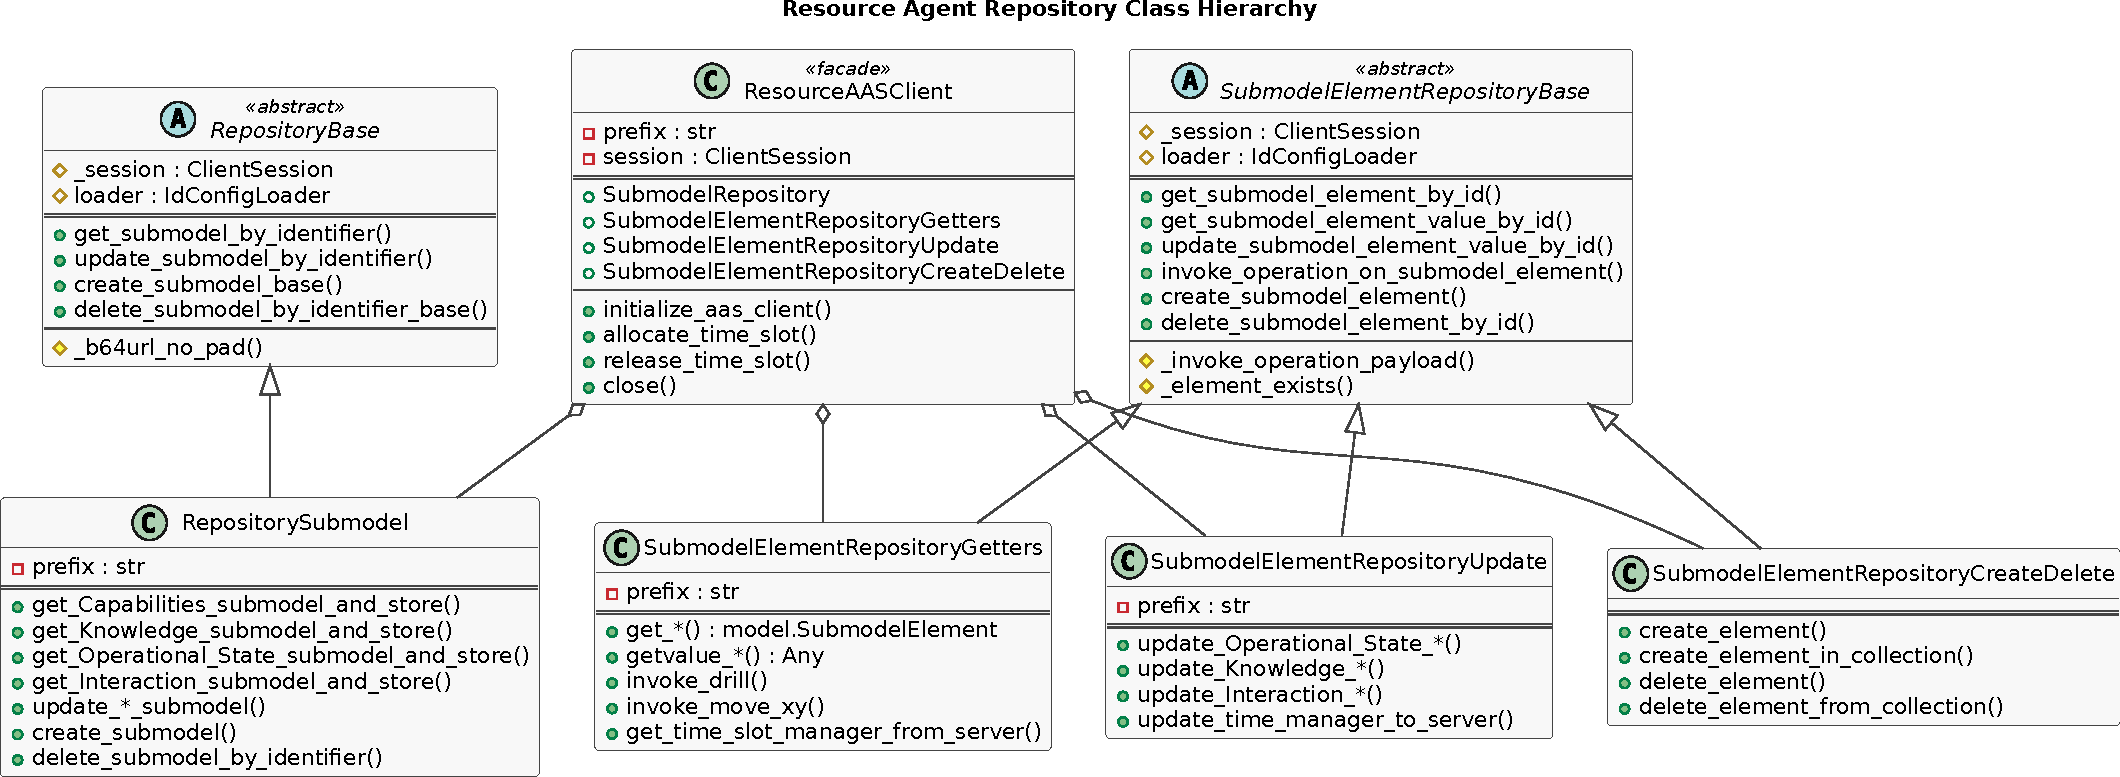
\includegraphics[width=24cm]{Images/repository_hierarchy.pdf}
    \caption{Resource Agent Repository Class Hierarchy}
    \label{fig:repository_architecture}
\end{figure}
\end{landscape}
\subsubsection{Base Classes}

\textbf{RepositoryBase} serves as the abstract foundation for Submodel-level operations. It encapsulates HTTP session management using aiohttp, Base64 URL-safe encoding for \ac{AAS} identifiers (as required by the BaSyx API), and JSON serialization using BaSyx SDK encoders. This class provides generic CRUD operations for retrieving, updating, creating, and deleting entire Submodels.

\textbf{SubmodelElementRepositoryBase} extends the base functionality for SubmodelElement-level operations. It handles path-based element access using dot notation for nested collections (e.g., \texttt{Collection.Property}), operation invocation with automatic payload construction, and idempotent element creation with existence checks.


\subsubsection{Specialized Repositories}

\textbf{RepositorySubmodel} inherits from RepositoryBase and provides Submodel-specific methods for each of the four ResourceAAS submodels. It includes a prefix injection mechanism that enables support for multiple resource instances (e.g., Drill\_1, Drill\_2) by dynamically modifying submodel identifiers.

\textbf{SubmodelElementRepositoryGetters} provides read-only access to submodel elements. It follows a dual naming convention: \texttt{get\_*()} methods return complete BaSyx model objects, while \texttt{getvalue\_*()} methods return only the element values. This class also provides operation invocation methods (\texttt{invoke\_drill()}, \texttt{invoke\_move\_xy()}) and utility methods like \texttt{get\_time\_slot\_manager\_from\_server()} for complex data retrieval.

\textbf{SubmodelElementRepositoryUpdate} provides write operations for modifying submodel element values. It mirrors the getter structure with update methods for each element type across all submodels.

\textbf{SubmodelElementRepositoryCreateDelete} handles element lifecycle management, supporting dynamic addition and removal of submodel elements during runtime.

\textbf{ResourceAASClient} acts as a facade that aggregates all repository instances. It is initialized with a resource prefix and provides a single entry point for agent behaviors to access \ac{AAS} data:

\begin{verbatim}
class ResourceAASClient:
    def __init__(self, prefix: str = ""):
        self.prefix = prefix
        
    async def initialize_aas_client(self):
        self.session = aiohttp.ClientSession()
        self.SubmodelRepository = RepositorySubmodel(self.session, self.prefix)
        self.SubmodelElementRepositoryGetters = SubmodelElementRepositoryGetters(
            self.session, self.prefix)
        self.SubmodelElementRepositoryUpdate = SubmodelElementRepositoryUpdate(
            self.session, self.prefix)
\end{verbatim}

This layered architecture ensures that the agent core remains decoupled from REST API details, facilitating testing and maintenance.

\subsection{Resource Agent Core}
\label{subsec:resource_agent_core}

The Resource Agent Core implements the \ac{BDI} reasoning cycle that enables autonomous behavior. This subsection describes the agent class structure, the AgentSpeak plans, and the SPADE behaviors that execute agent actions. Figure~\ref{fig:resource_agent_core} illustrates the class architecture.

    

\begin{figure}[p]
    \centering
    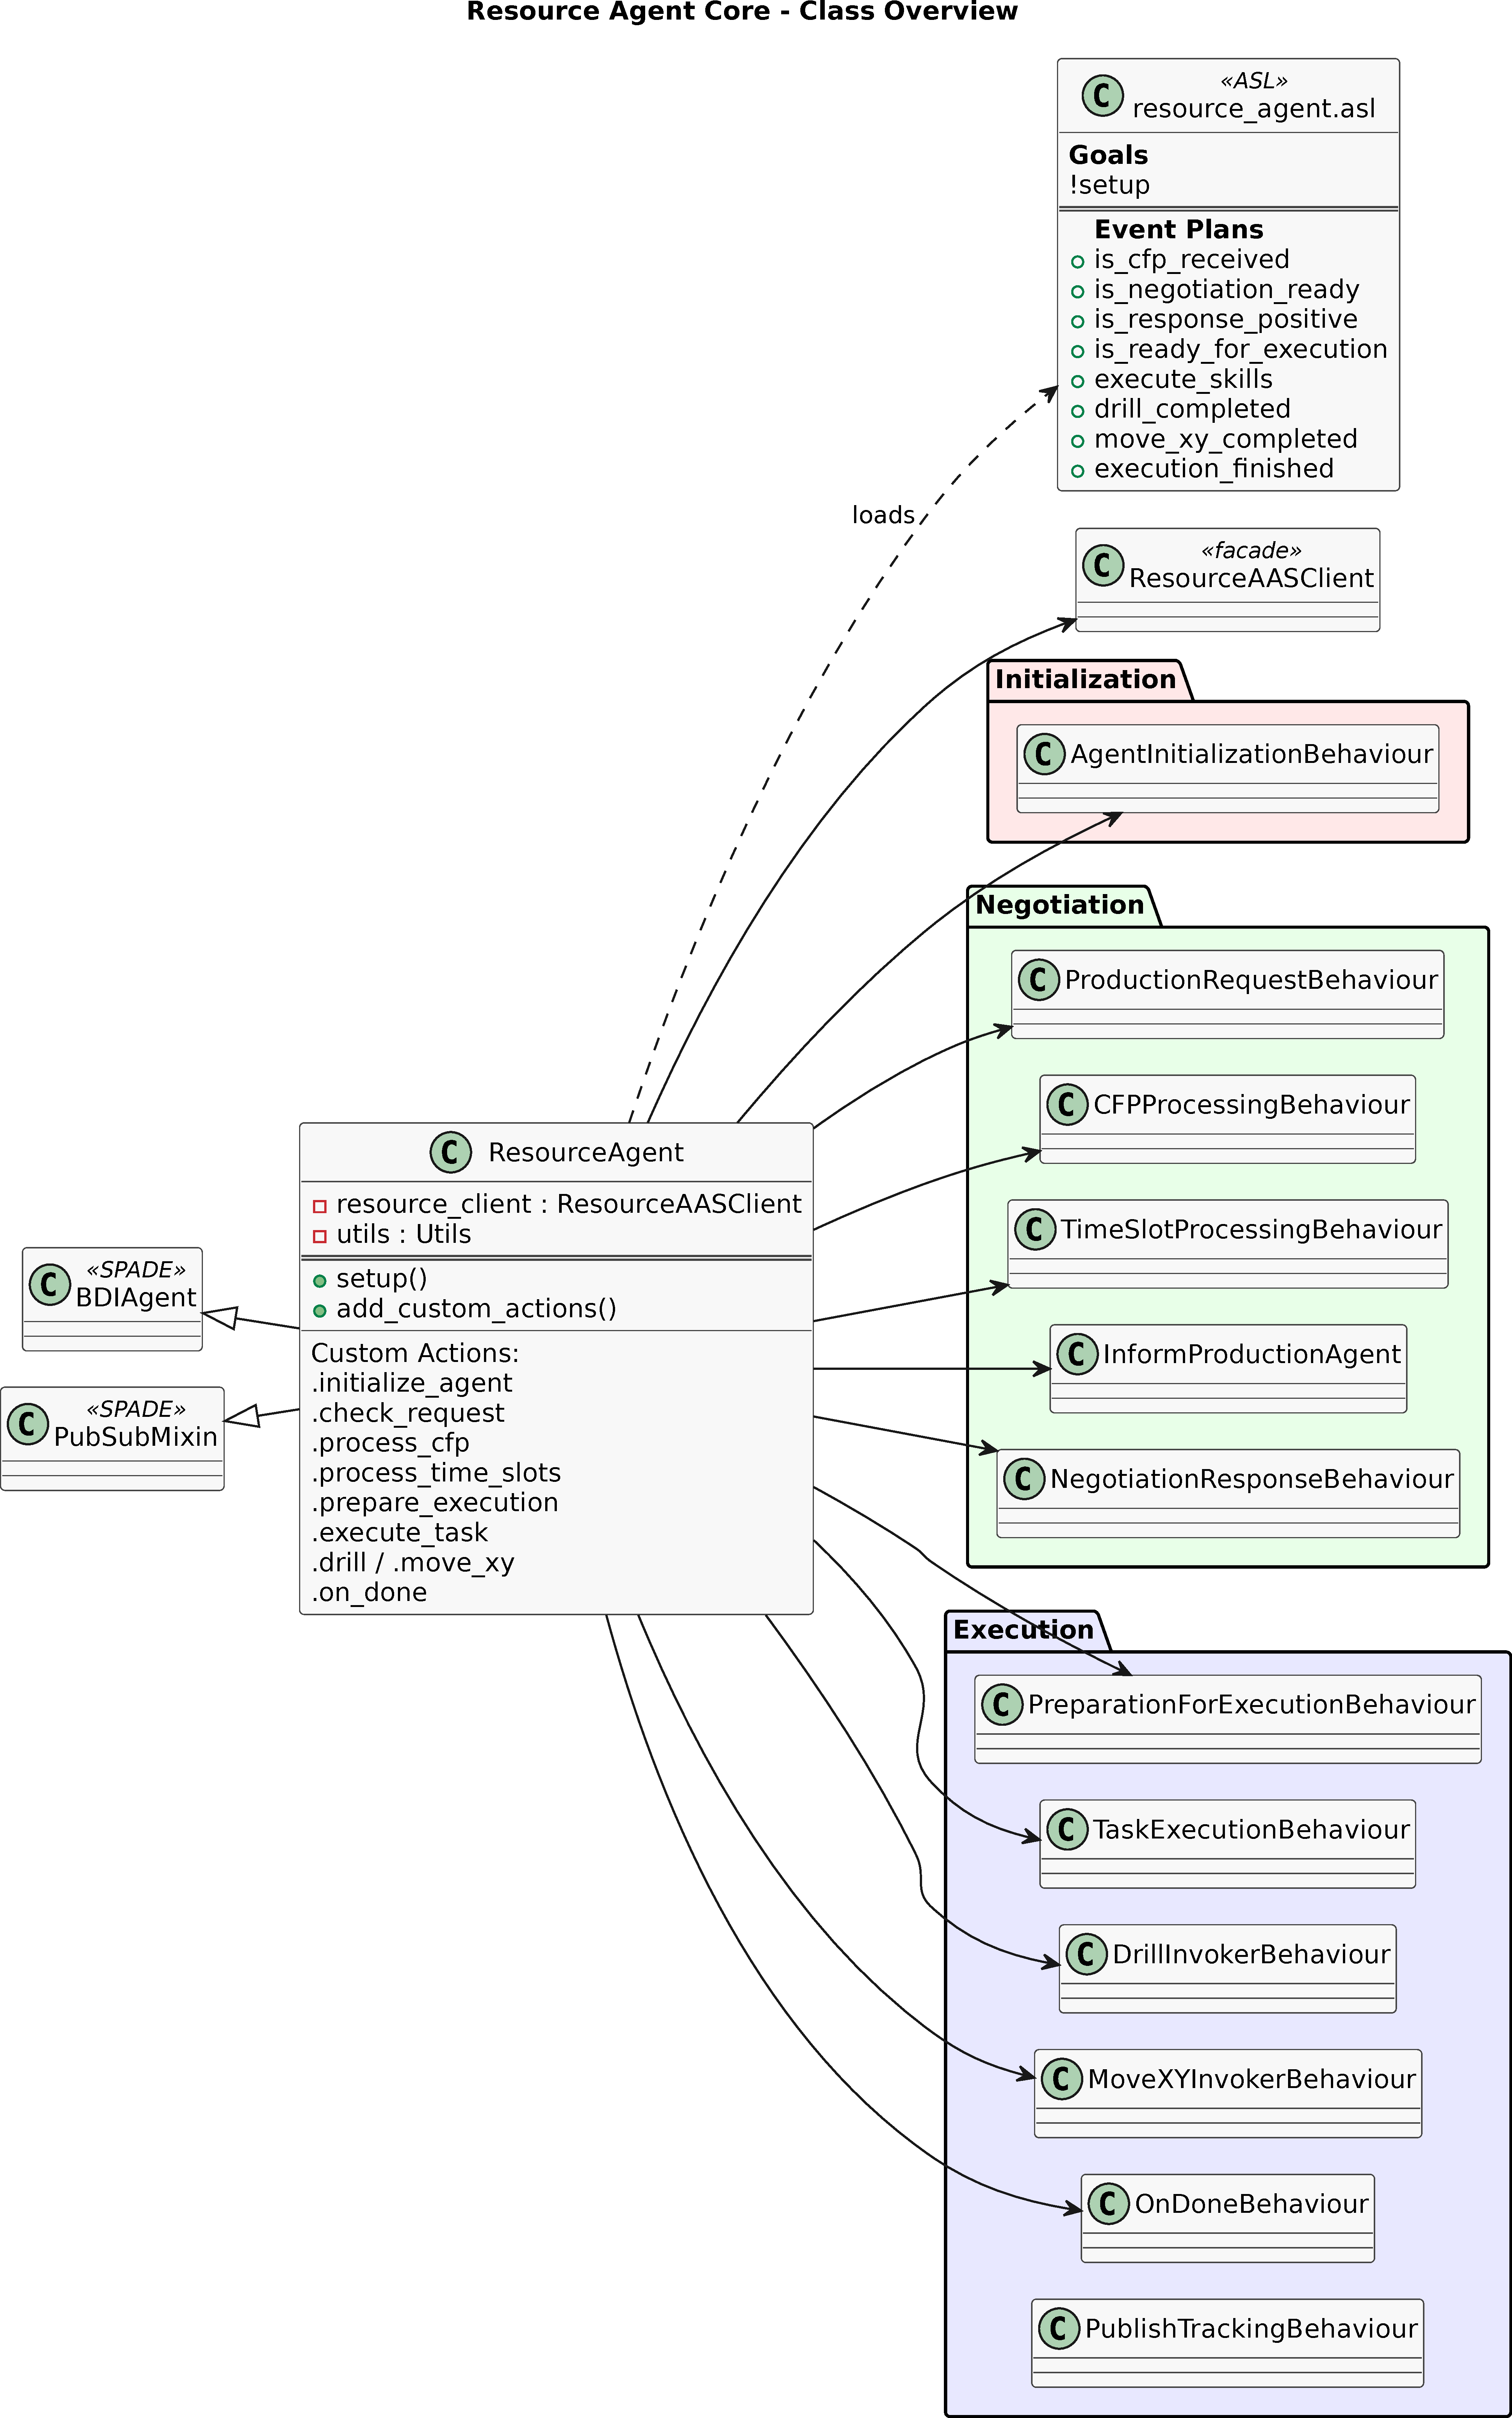
\includegraphics[width=0.95\textwidth]{Images/Resource_Agent_Core_Simple.pdf}
    \caption{Resource Agent Core Class Architecture}
    \label{fig:resource_agent_core}
\end{figure}

\subsubsection{ResourceAgent Class}

The \texttt{ResourceAgent} class extends both \texttt{BDIAgent} and \texttt{PubSubMixin} from the SPADE framework. This dual inheritance combines AgentSpeak-based reasoning with \ac{XMPP} publish-subscribe messaging. The agent maintains a reference to the \texttt{ResourceAASClient} for \ac{AAS} communication and registers custom actions that map AgentSpeak plan actions to SPADE behaviors.

Custom actions are registered in the \texttt{add\_custom\_actions()} method. Each action corresponds to a specific behavior class. For example, when an AgentSpeak plan executes \texttt{.drill}, the agent instantiates and adds a \texttt{DrillInvokerbehavior} to its execution queue.
\subsubsection{AgentSpeak Plans}

The agent's reactive behavior is defined in the \texttt{resource\_agent.asl} file using AgentSpeak syntax. Plans follow the pattern \texttt{+trigger : context <- body}, where the trigger is a belief change, the context is an optional condition, and the body contains actions to execute.

\textbf{Initialization.} The agent starts with the goal \texttt{!setup}, which triggers belief loading from \ac{AAS} submodels and initiates request listening.

\textbf{Negotiation Plans.} When a Call-For-Proposal arrives, the belief \texttt{is\_cfp\_received(true)} triggers validation plans that check time slots, current state, and skill constraints. The result is published back to the ProductionAAS.

\textbf{Execution Plans.} Upon receiving a positive negotiation response, execution plans coordinate the operation sequence. For drilling tasks, the agent first executes \texttt{move\_xy}, then upon completion triggers \texttt{drill}. Context conditions ensure correct sequencing:
\begin{verbatim}
+move_xy_completed(true) : current_operation(drill) <-
    .drill.
\end{verbatim}
\subsubsection{SPADE behaviors}

behaviors implement the actual logic for each agent action. They are organized into three categories:

\textbf{Initialization behaviors.} \texttt{AgentInitializationbehavior} reads beliefs from all four submodels concurrently using \texttt{asyncio.gather()}, populating the agent's belief base with current state, supported skills, constraints, and time slot availability.

\textbf{Negotiation behaviors.} These behaviors handle the Contract Net Protocol interaction:
\begin{itemize}
    \item \texttt{ProductionRequestbehavior}: Listens for CFP messages via \ac{XMPP} PubSub
    \item \texttt{TimeSlotProcessingbehavior}: Validates requested time slot availability
    \item \texttt{CFPProcessingbehavior}: Validates state, skills, and constraints against the CFP
    \item \texttt{InformProductionAgent}: Sends the negotiation response with any violations
    \item \texttt{NegotiationResponsebehavior}: Processes the ProductionAAS decision
\end{itemize}

\textbf{Execution behaviors.} These behaviors execute the actual operations:
\begin{itemize}
    \item \texttt{PreparationForExecutionbehavior}: Prepares the resource (e.g., allocates time slot)
    \item \texttt{TaskExecutionbehavior}: Determines which skill to execute based on the CFP
    \item \texttt{DrillInvokerbehavior}: Invokes the drill operation via the \ac{AAS} API
    \item \texttt{MoveXYInvokerbehavior}: Invokes the positioning operation
    \item \texttt{PublishTrackingbehavior}: Publishes execution status events
    \item \texttt{OnDonebehavior}: Performs cleanup and releases allocated resources
\end{itemize}


\subsubsection{Agent State Machine}

Figure~\ref{fig:resource_agent_statemachine} shows the complete state machine of the ResourceAgent, illustrating the flow from initialization through negotiation to execution.

\begin{figure}[p]
    \centering
    \makebox[\textwidth][c]{%
        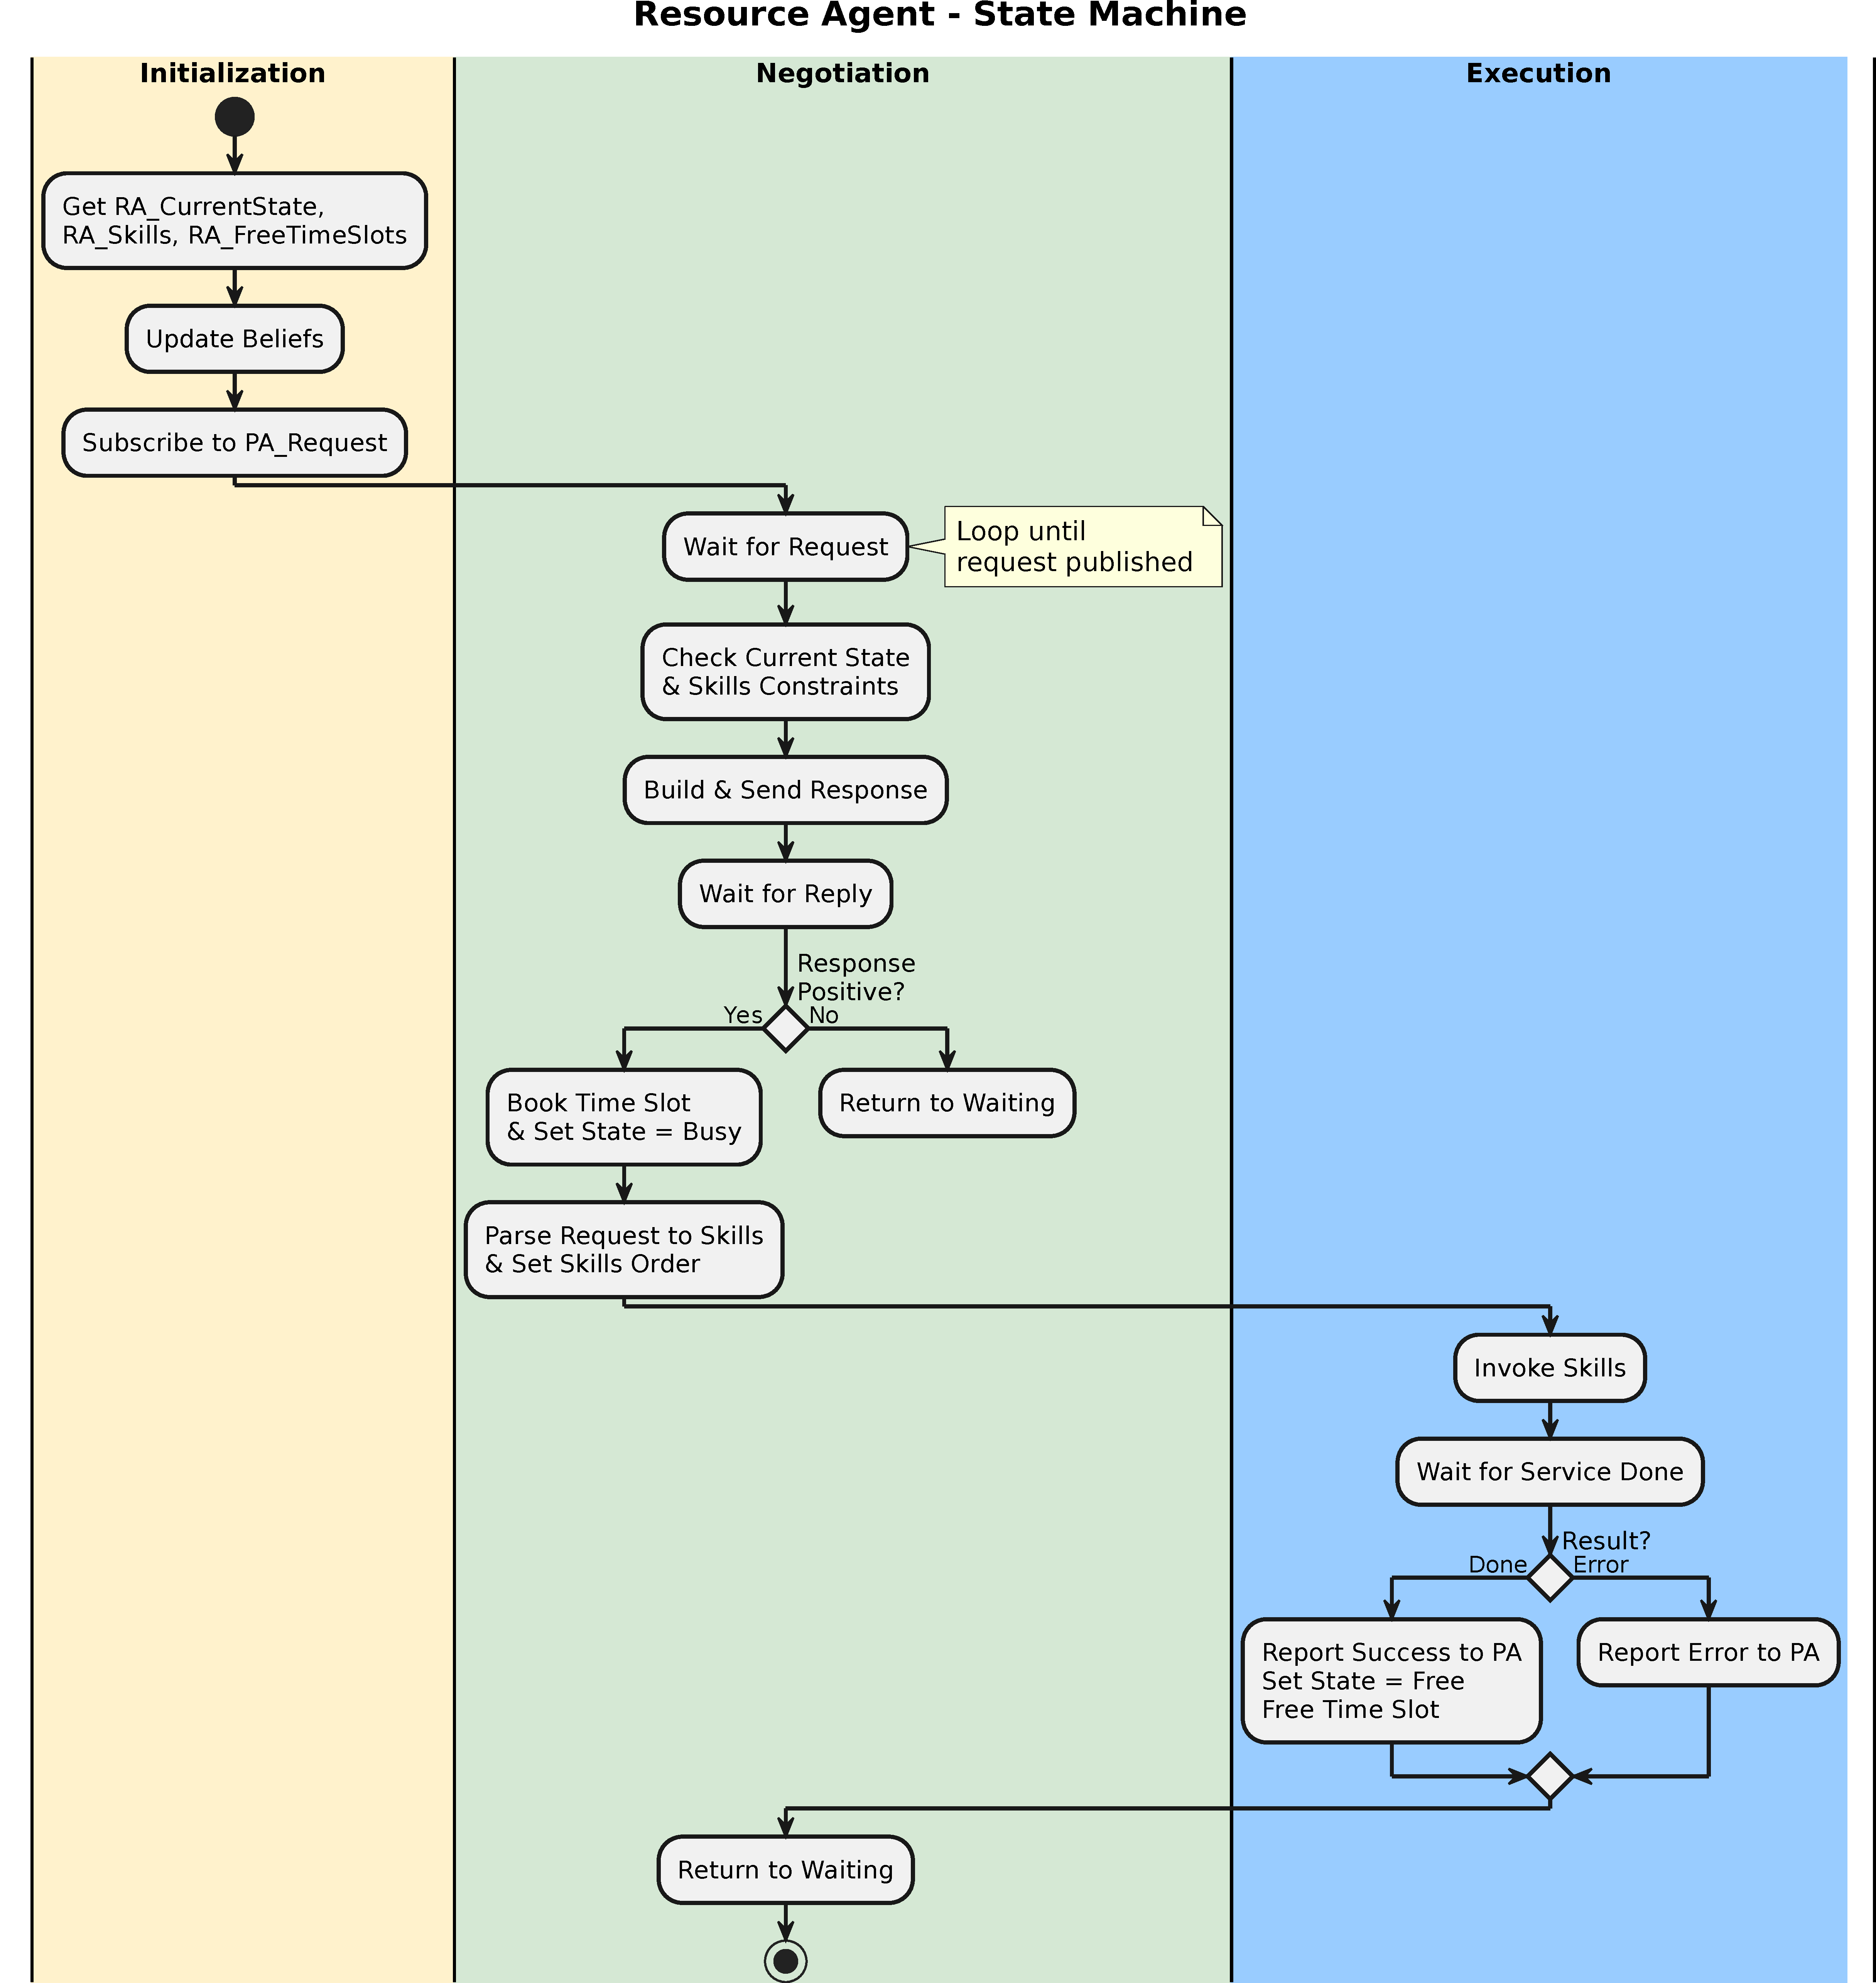
\includegraphics[width=1.3\textwidth]{Images/Resource_Agent_State_Machine.pdf}%
    }
    \caption{Resource Agent State Machine}
    \label{fig:resource_agent_statemachine}
\end{figure}
The state machine comprises six main phases: initialization (loading beliefs from submodels), waiting (listening for CFP requests), CFP processing (validating the request), negotiation response handling (waiting for ProductionAAS decision), execution (performing the requested operation), and cleanup (releasing resources and returning to waiting state).

\subsection{Resource Simulators}
\label{subsec:resource_simulators}
To enable testing and validation of the ResourceAAS without physical hardware, the system includes discrete-event simulators that emulate the behavior of drill machines and positioning systems. These simulators implement the same HTTP endpoints as real machine controllers, allowing seamless integration with the \ac{AAS} infrastructure via the invocationDelegation pattern.

\subsubsection{Simulator Architecture}

Each simulator is implemented as a standalone FastAPI application that combines discrete-event simulation with asynchronous HTTP handling. The architecture uses SimPy~\cite{simpy}, a process-based discrete-event simulation framework for Python, to model machine operations with realistic timing behavior. Figure~\ref{fig:simulator_architecture} illustrates the simulator integration.

\begin{figure}[ht]
    \centering
    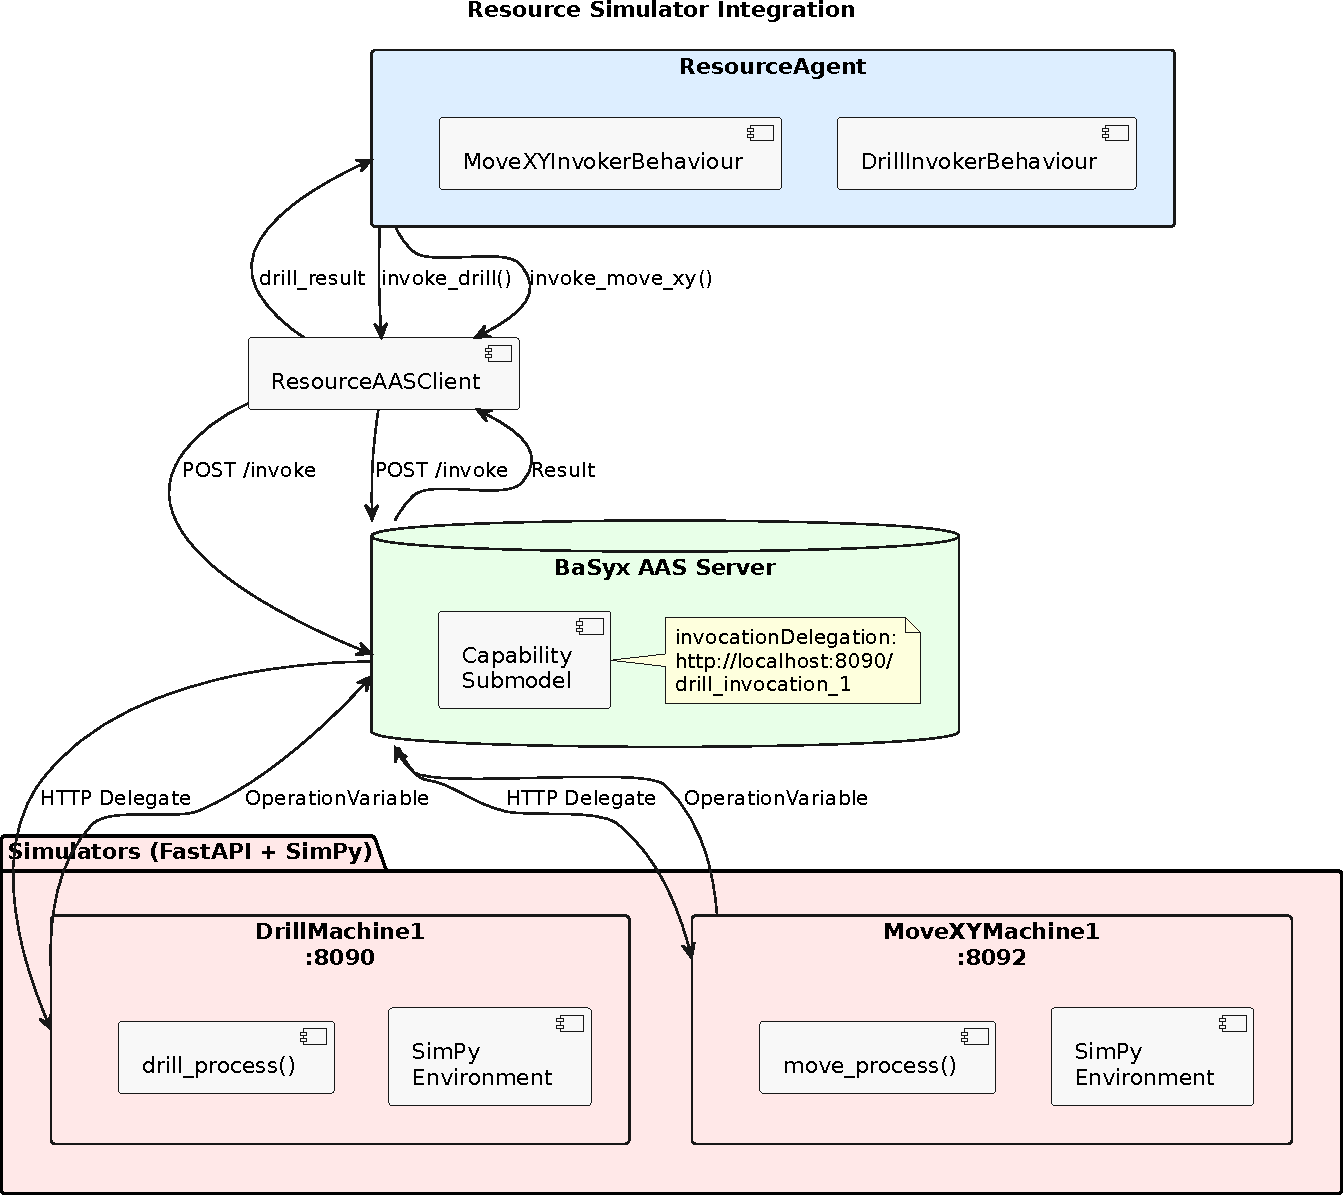
\includegraphics[width=0.95\textwidth]{Images/simulator_architecture.pdf}
    \caption{Resource Simulator Integration Architecture}
    \label{fig:simulator_architecture}
\end{figure}

The simulators expose HTTP endpoints that match the invocationDelegation URLs defined in the Capability Submodel Operations. When the BaSyx server receives an operation invocation request, it forwards the call to the simulator endpoint, which executes the simulated operation and returns \ac{AAS}-compliant results.
\subsubsection{Drill Machine Simulator}

The \texttt{DrillMachine} simulator models drilling operations with configurable speed factors and setup times. Key components include:

\textbf{Machine State.} The simulator maintains state information including current operational status (Idle/Drilling), last drill depth, jobs completed, and cumulative drill time.

\textbf{Drill Process.} The SimPy process calculates drill duration based on depth and RPM parameters using a simple simulation formula:
\begin{equation}
t_{drill} = t_{setup} + depth \times factor_{speed} \times \frac{1500}{RPM}
\end{equation}
This formula scales drill time linearly with depth and inversely with RPM, plus a fixed setup time. It is not based on real machining physics but provides a reasonable approximation for simulation purposes, where higher RPM values result in faster drilling and deeper holes require proportionally more time.

\textbf{Resource Management.} A SimPy Resource with capacity 1 ensures mutual exclusion, preventing concurrent operations on the same machine.

\subsubsection{MoveXY Simulator}

The \texttt{MoveXYMachine} simulator models 2D positioning operations. It tracks the current position and calculates movement time based on Euclidean distance:
\begin{equation}
t_{move} = t_{setup} + \sqrt{(x_{target} - x_{current})^2 + (y_{target} - y_{current})^2} \times factor_{move}
\end{equation}
Similar to the drill formula, this is a simplified simulation model where movement time scales linearly with distance traveled, plus a fixed setup time. The simulator maintains position state between operations, enabling realistic simulation of sequential movements.

\subsubsection{AAS Integration}

Simulators integrate with the \ac{AAS} infrastructure through the invocationDelegation pattern:

\begin{enumerate}
    \item The ResourceAgent behavior calls \texttt{invoke\_drill()} on the ResourceAASClient
    \item The client sends an invocation request to the BaSyx server
    \item BaSyx reads the invocationDelegation qualifier from the Operation element
    \item BaSyx forwards the request to the simulator endpoint\\
    (e.g., \texttt{http://localhost:8090/drill\_invocation\_1})
    \item The simulator executes the SimPy process and returns \ac{AAS}-compliant OperationVariable results
    \item The response propagates back through BaSyx to the agent
\end{enumerate}

This design enables transparent switching between simulators and real machine controllers by modifying only the invocationDelegation URL in the Capability Submodel, without changes to agent code.

\subsubsection{Simulator Instances}

The system includes four simulator instances to support the multi-resource scenario:

\begin{table}[ht]
\centering
\caption{Resource Simulator Configuration}
\label{tab:simulator_config}
\begin{tabular}{llll}
\toprule
\rowcolor{headerblue}
\textcolor{white}{Simulator} & \textcolor{white}{Port} & \textcolor{white}{Endpoint} & \textcolor{white}{Resource} \\
\midrule
DrillMachine1 & 8090 & /drill\_invocation\_1 & Drill\_1 \\
DrillMachine2 & 8091 & /drill\_invocation\_2 & Drill\_2 \\
MoveXYMachine1 & 8092 & /movexy\_invocation\_1 & Drill\_1 \\
MoveXYMachine2 & 8093 & /movexy\_invocation\_2 & Drill\_2 \\
\bottomrule
\end{tabular}
\end{table}

Each drill machine resource has an associated MoveXY simulator, reflecting the physical configuration where positioning and drilling are separate actuators on the same machine.


\section{Production Agent Concept}
\label{sec:production_agent}

The ProductionAAS orchestrates the manufacturing process by coordinating resource agents, managing process plans, and tracking execution progress. Unlike the ResourceAAS which represents physical assets, the ProductionAAS operates at the product level, initiating negotiations with resources and monitoring task completion. This section describes the Production Agent architecture, submodels, and its dual-core design for execution and negotiation.

\subsection{Production Agent Overview}
\label{subsec:production_overview}

The ProductionAAS follows a similar architectural pattern to the ResourceAAS but serves a different purpose in the system hierarchy. While ResourceAAS agents represent manufacturing capabilities, the ProductionAAS represents production orders and coordinates the execution of process plans across multiple resources. Figure~\ref{fig:production_components} illustrates the Production Agent component structure.
\begin{figure}[p]
    \centering
    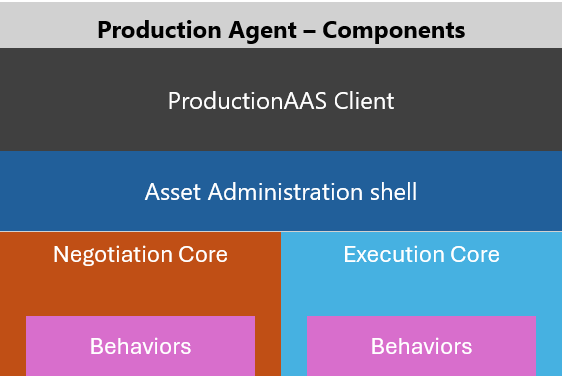
\includegraphics[width=0.9\textwidth]{Images/production_components.png}
    \caption{Production Agent Component Structure}
    \label{fig:production_components}
\end{figure}

\textbf{ProductionAASClient.} Similar to the ResourceAASClient, this facade aggregates repository classes for accessing Production submodels. It provides methods for reading process plans, updating execution state, and managing interface configurations.


\textbf{Asset Administration Shell.} The Production \ac{AAS} contains submodels that describe the production order rather than physical capabilities. These include the Process Plan defining the sequence of operations, Execution Tracking for monitoring progress, and Interface Endpoints for communication configuration. The shell is deployed to the same BaSyx environment as ResourceAAS instances, enabling unified access through the \ac{AAS} API.

\textbf{Dual-Core Agent Architecture.} The Production Agent implements a separation of concerns through two specialized agent cores:
\begin{itemize}
    \item \textbf{Execution Core}: Handles user requests, monitors execution progress, and updates the Execution Tracking submodel based on events from resource agents.
    \item \textbf{Negotiation Core}: Manages the Contract Net Protocol interaction with resource agents, collecting responses and selecting the best-fit resource for task execution.
\end{itemize}

This separation allows independent scaling and clearer responsibility boundaries compared to a monolithic agent design.
\begin{figure}[p]
    \centering
    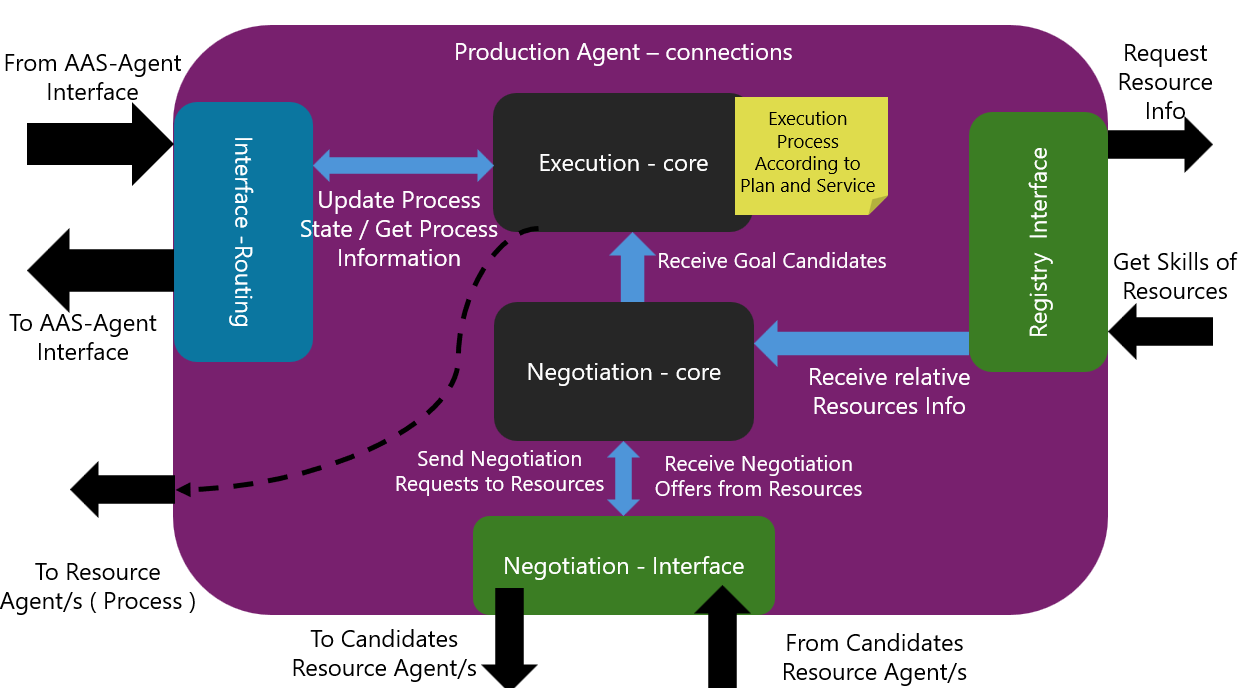
\includegraphics[width=0.9\textwidth]{Images/production_Internal.png}
    \caption{Production Agent Internal Architecture}
    \label{fig:production_internal}
\end{figure}


\subsection{Production Agent Submodels}
\label{subsec:production_submodels}
The ProductionAAS contains three submodels that support process definition, execution monitoring, and communication configuration.

\subsubsection{Process Plan Submodel}

The Process Plan Submodel defines the sequence of operations required to fulfill a production order. It uses a graph-based representation with nodes, edges, and control flow elements. Figure~\ref{fig:sm_process_plan} shows the structure of this submodel.

\textbf{Nodes.} A SubmodelElementCollection containing Property elements for each operation in the process. In the drill machine scenario, this includes:
\begin{itemize}
    \item \texttt{Move\_Node}: Positioning operation to coordinates X, Y
    \item \texttt{Drill\_Node}: Drilling operation with depth and RPM parameters
\end{itemize}

\textbf{Edges.} A SubmodelElementCollection defining the execution sequence between nodes (e.g., ``Move\_Node to Drill\_Node'').

\textbf{Entry\_Point / Exit\_Point.} Properties indicating the first and last nodes in the process plan, enabling the Execution Core to determine where to begin and when execution is complete.

\textbf{Preconditions / Postconditions.} Properties defining the required state before execution can begin and the expected state after completion.

\textbf{Required\_Capabilities.} A list of capabilities needed to execute the process plan (e.g., ``[Drill\_Capability, MoveXY\_Capability]''). The Negotiation Core uses this to filter resource agents during CFP broadcast.


\begin{landscape}
\begin{figure}[p]
    \centering
    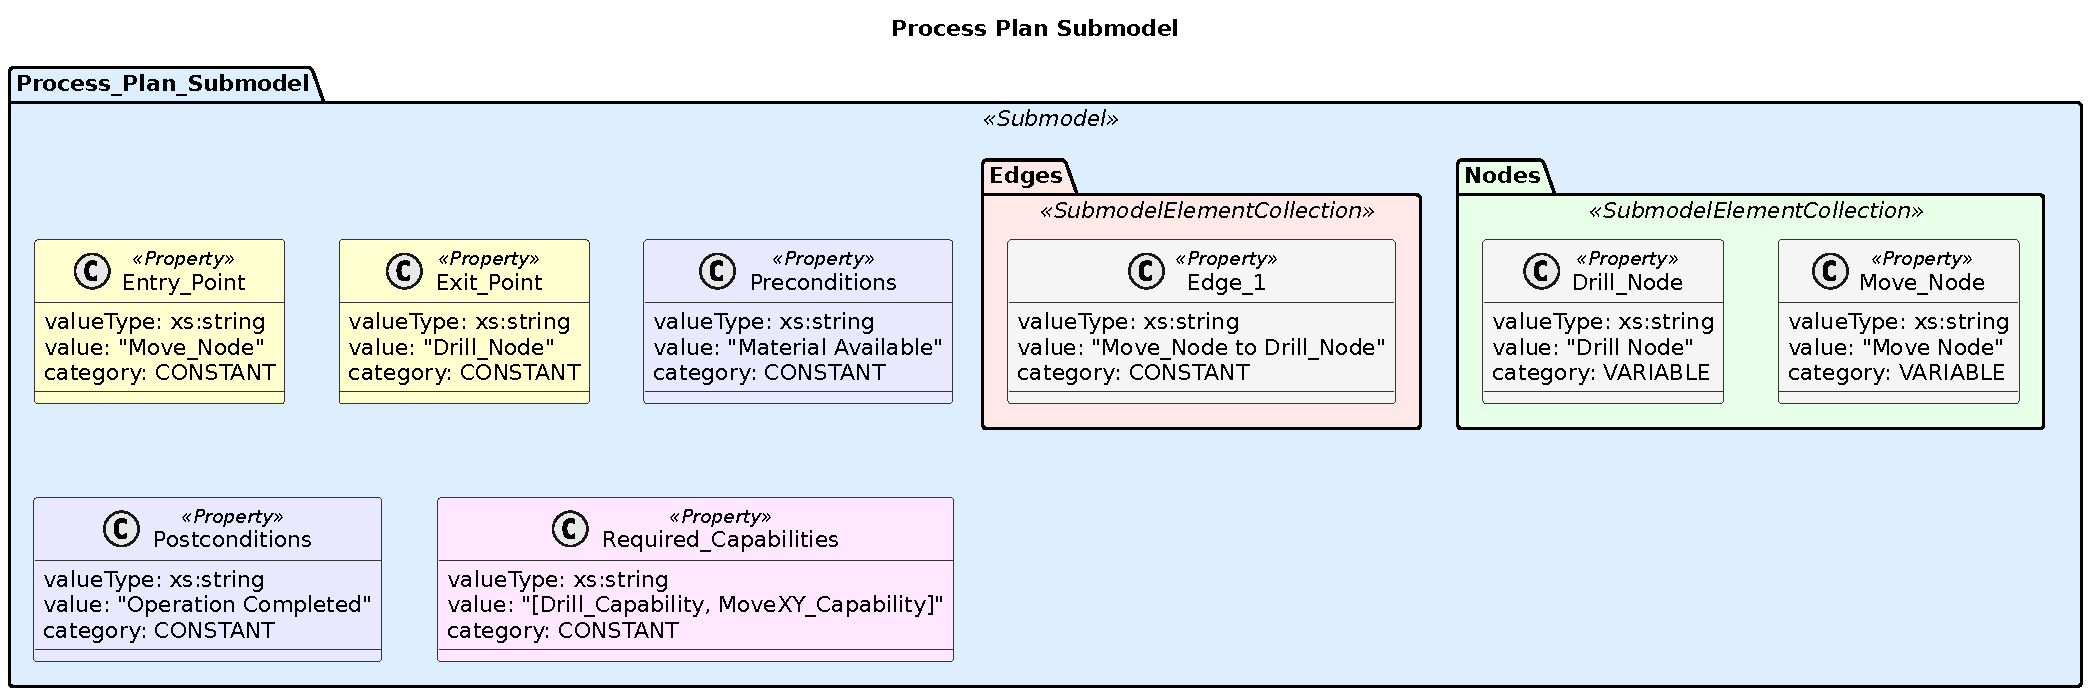
\includegraphics[width=24cm]{Images/sm_process_plan.pdf}
    \caption{Process Plan Submodel Structure}
    \label{fig:sm_process_plan}
\end{figure}
\end{landscape}
\subsubsection{Execution Tracking Submodel}

The Execution Tracking Submodel provides real-time visibility into process execution. It is updated by the Execution Core as resource agents report progress. Figure~\ref{fig:sm_execution_tracking} shows the structure.

\begin{figure}[p]
    \centering
    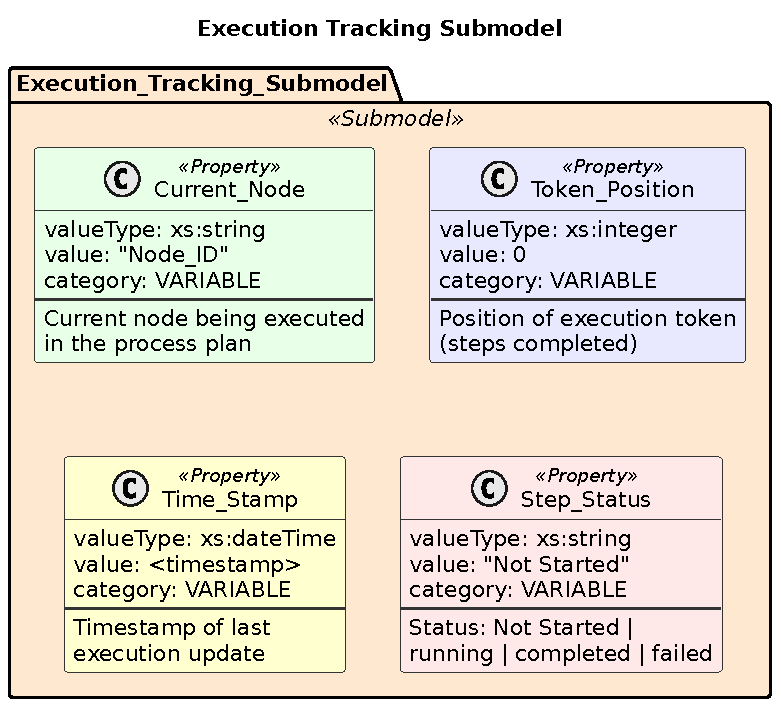
\includegraphics[width=0.9\textwidth]{Images/sm_execution_tracking.pdf}
    \caption{Execution Tracking Submodel Structure}
    \label{fig:sm_execution_tracking}
\end{figure}

\textbf{Current\_Node.} The node currently being executed in the process plan, updated when resource agents publish tracking events.

\textbf{Token\_Position.} An integer indicating how many steps have been completed, implementing a simple Petri net-style token tracking mechanism.

\textbf{Time\_Stamp.} The timestamp of the last execution update, providing temporal context for monitoring systems.

\textbf{Step\_Status.} The status of the current operation: ``Not Started'', ``running'', ``completed'', or ``failed''.

\subsubsection{Interface Endpoints Submodel}

The Interface Endpoints Submodel as in figure~\ref{fig:sm_interface_endpoints} contains configuration for external communication, similar to the Interaction Submodel in ResourceAAS but focused on command invocation endpoints.

\begin{figure}[p]
    \centering
    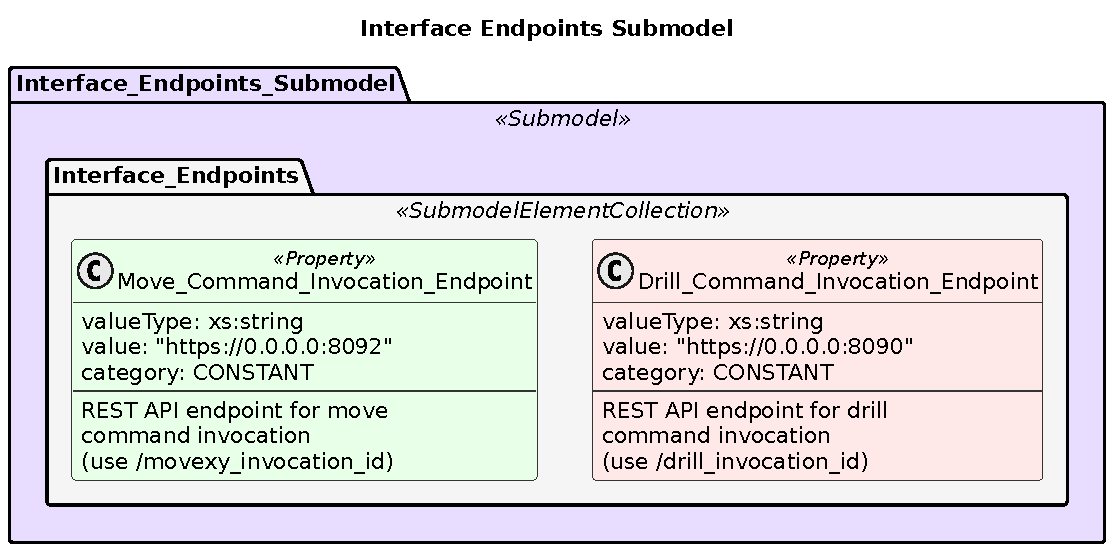
\includegraphics[width=0.9\textwidth]{Images/sm_interface_endpoints.pdf}
    \caption{Interface Endpoints Submodel Structure}
    \label{fig:sm_interface_endpoints}
\end{figure}

\textbf{Endpoints Collection.} Contains properties for:
\begin{itemize}
    \item \texttt{Drill\_Command\_Invocation\_Endpoint}: Base URL for drill operation invokers
    \item \texttt{Move\_Command\_Invocation\_Endpoint}: Base URL for movement operation invokers
\end{itemize}




\subsection{Production Agent Execution Core}
\label{subsec:production_execution}

The Execution Core manages the lifecycle of production requests from receipt through completion. It operates as a SPADE agent extending both \texttt{Agent} and \texttt{PubSubMixin} for \ac{XMPP} communication. Figure~\ref{fig:execution_core} illustrates the class architecture.

\begin{landscape}
    

\begin{figure}[p]
    \centering
    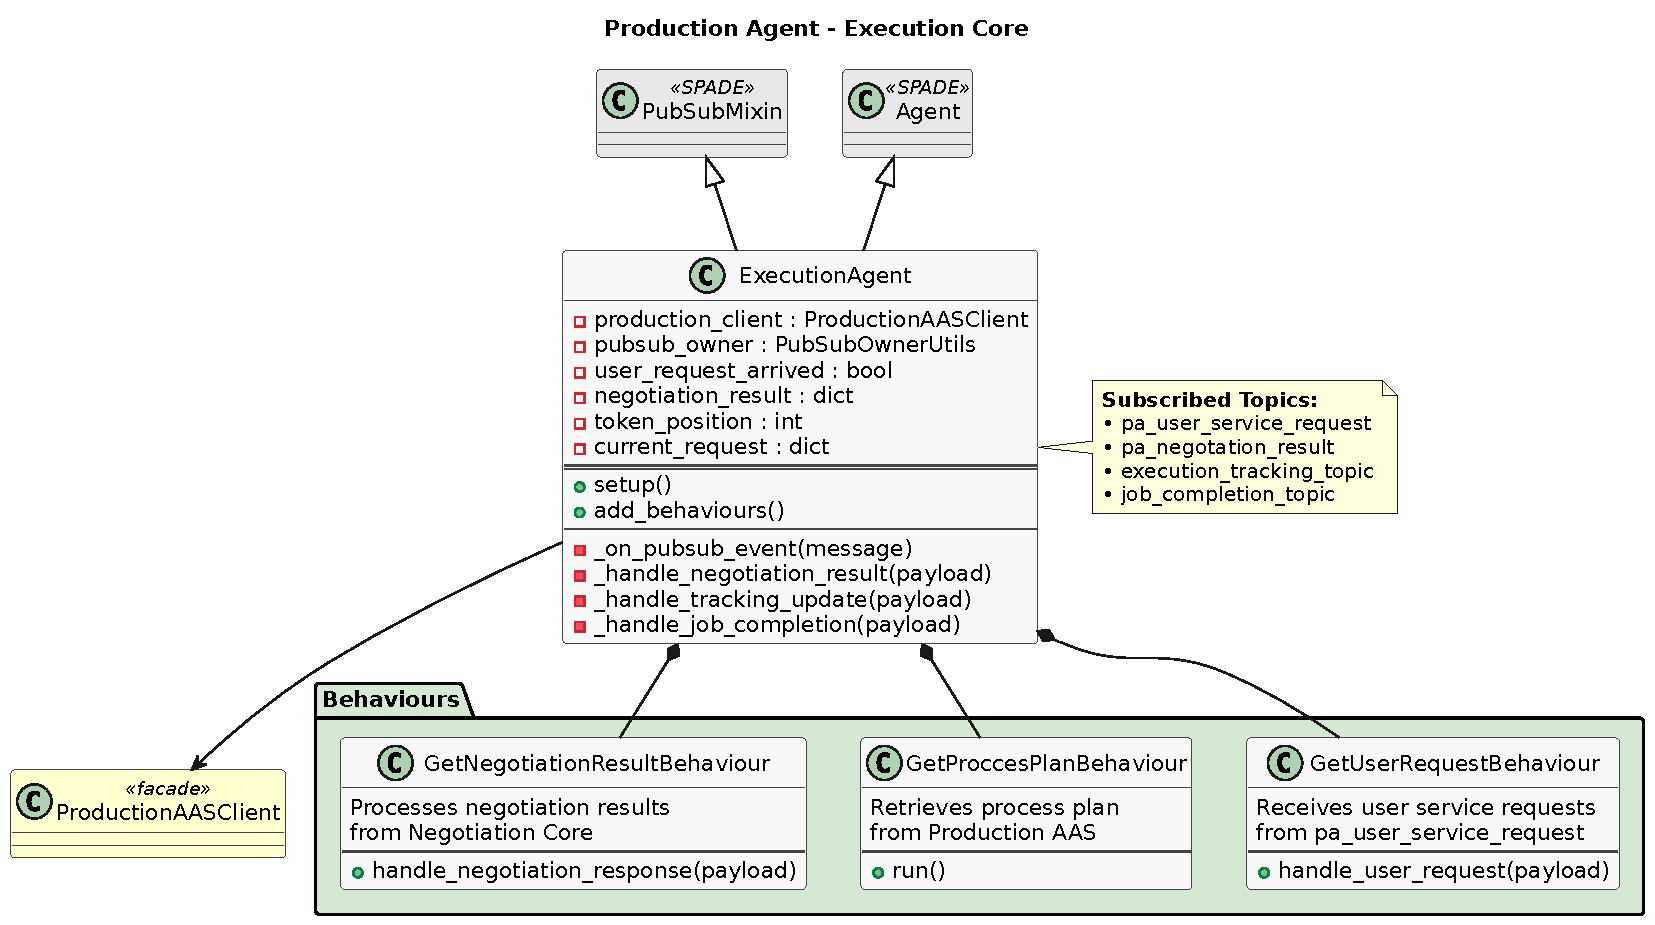
\includegraphics[width=24cm]{Images/execution_core_simple.pdf}
    \caption{Execution Core Class Architecture}
    \label{fig:execution_core}
\end{figure}
\end{landscape}
\subsubsection{ExecutionAgent Class}

The \texttt{ExecutionAgent} class serves as the central coordinator for production execution. It maintains several key attributes:

\begin{itemize}
    \item \texttt{production\_client}: Reference to the ProductionAASClient for accessing submodel data
    \item \texttt{pubsub\_owner}: Utility for managing \ac{XMPP} PubSub node ownership and subscriptions
    \item \texttt{negotiation\_result}: Stores the selected resource and parameters from negotiation
    \item \texttt{token\_position}: Tracks execution progress through the process plan (Petri net-style counter)
    \item \texttt{current\_request}: Stores the active production request for reference during tracking
\end{itemize}

During setup, the agent initializes the ProductionAASClient and subscribes to four \ac{XMPP} topics:
\begin{itemize}
    \item \texttt{pa\_user\_service\_request}: Receives new production requests
    \item \texttt{pa\_negotation\_result}: Receives negotiation outcomes from the Negotiation Core
    \item \texttt{execution\_tracking\_topic}: Receives progress updates from resource agents
    \item \texttt{job\_completion\_topic}: Receives task completion notifications
\end{itemize}

\subsubsection{Event Handling}

The \texttt{\_on\_pubsub\_event()} method routes incoming messages to appropriate handlers based on the topic:

\textbf{User Request Handling.} When a message arrives on \texttt{pa\_user\_service\_request}, the agent delegates to \texttt{GetUserRequestbehavior}, which parses the CFP message and forwards it to the Negotiation Core.

\textbf{Negotiation Result Handling.} The \texttt{\_handle\_negotiation\_result()} method processes the selected resource information, logs the negotiation summary, and triggers execution preparation.

\textbf{Tracking Update Handling.} The \texttt{\_handle\_tracking\_update()} method receives progress events from resource agents during execution. For each update, it increments the token position, updates the Execution Tracking Submodel via the ProductionAASClient, and logs the operation status.

\textbf{Job Completion Handling.} The \texttt{\_handle\_job\_completion()} method finalizes the production run by logging completion status and saving execution reports.

\subsubsection{behaviors}

The Execution Core uses three behaviors to handle different aspects of request processing:

\textbf{GetUserRequestbehavior.} Receives and parses user service requests from the \texttt{pa\_user\_service\_request} topic. It extracts the skill requirements, time slot preferences, and input parameters, then publishes the request to the Negotiation Core via \texttt{pa\_execution\_service\_topic}.

\textbf{GetProccesPlanbehavior.} Retrieves the process plan from the Production AAS, providing the Execution Core with information about the sequence of operations, entry/exit points, and required capabilities.

\textbf{GetNegotiationResultbehavior.} Processes negotiation results received from the Negotiation Core. Upon receiving a positive result with a selected resource, it prepares the execution context and waits for tracking updates as the resource agent executes the task.
\subsection{Production Agent Negotiation Core}
\label{subsec:production_negotiation}

The Negotiation Core implements the Contract Net Protocol initiator role, broadcasting Call-For-Proposals to resource agents and selecting the best candidate for task execution. Like the Execution Core, it operates as a SPADE agent with \ac{XMPP} publish-subscribe capabilities. Figure~\ref{fig:negotiation_core} illustrates the class architecture.

\begin{landscape}
\begin{figure}[p]
    \centering
    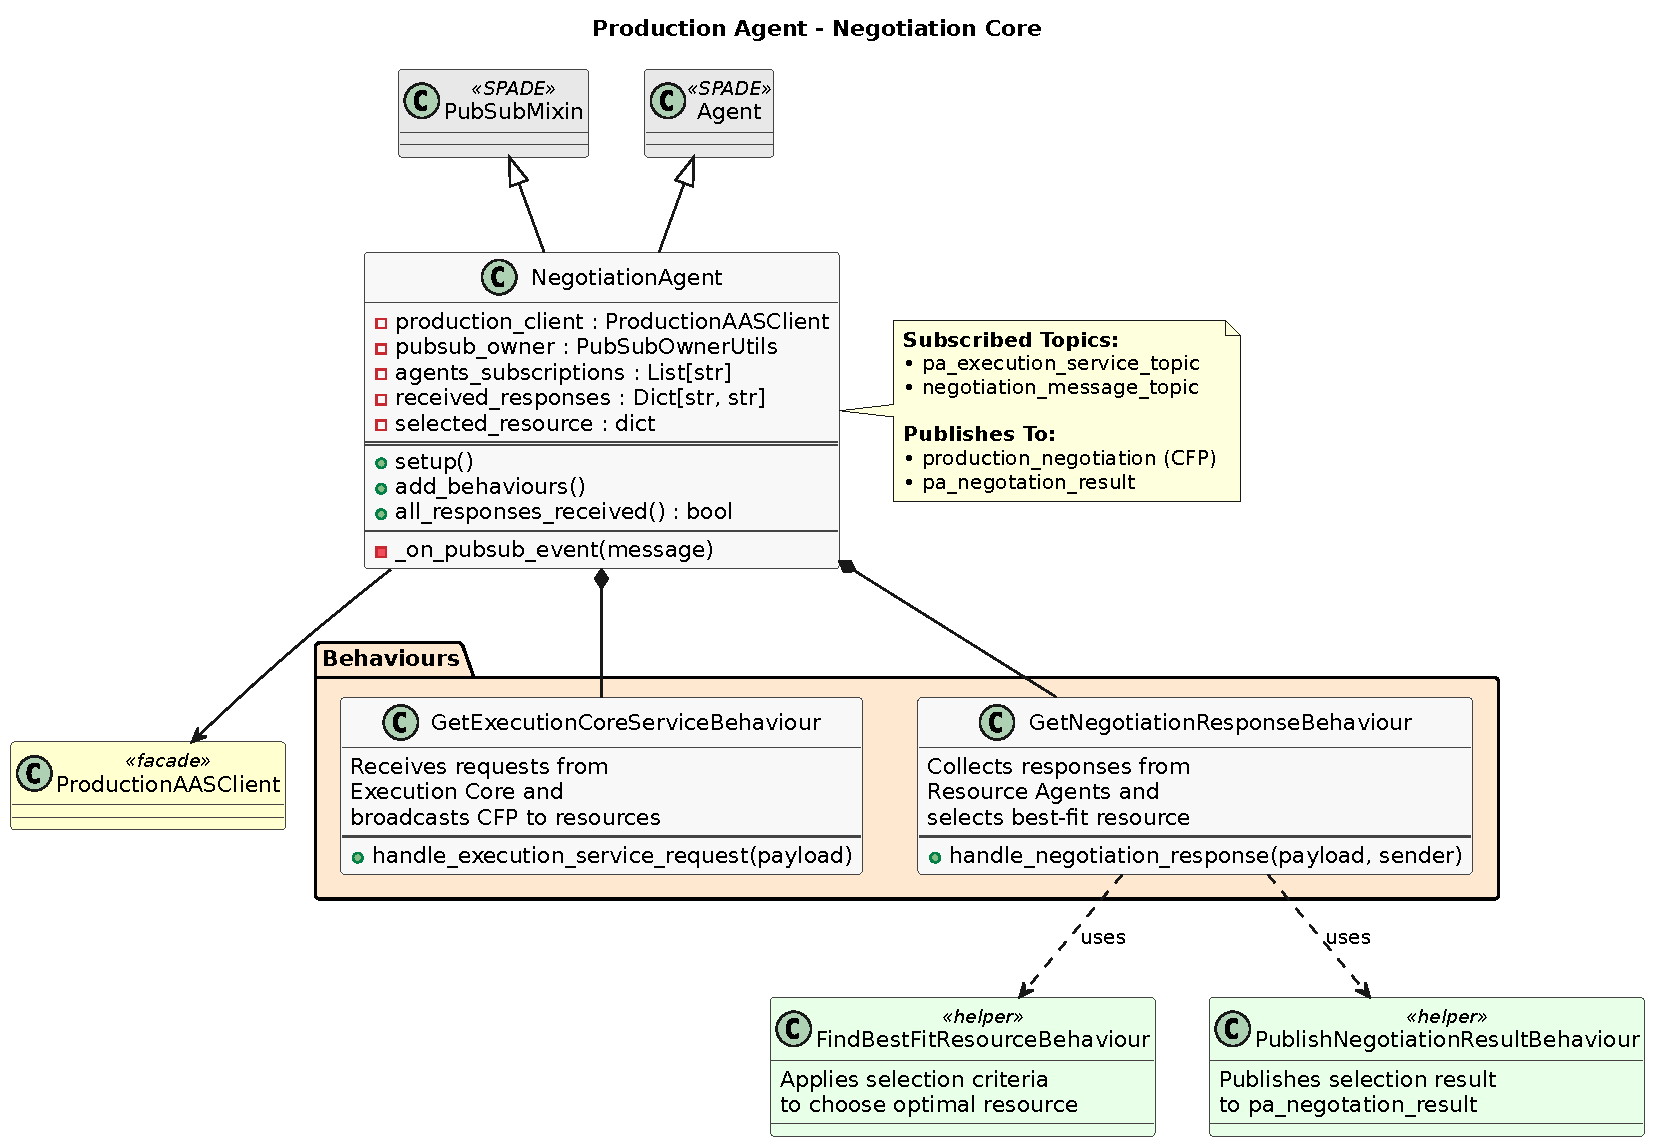
\includegraphics[width=23cm]{Images/negotiation_core_simple.pdf}
    \caption{Negotiation Core Class Architecture}
    \label{fig:negotiation_core}
\end{figure}
\end{landscape}
\subsubsection{NegotiationAgent Class}

The \texttt{NegotiationAgent} class manages the negotiation process with resource agents. It maintains several key attributes:

\begin{itemize}
    \item \texttt{production\_client}: Reference to the ProductionAASClient for accessing submodel data
    \item \texttt{pubsub\_owner}: Utility for querying \ac{XMPP} PubSub node subscribers
    \item \texttt{agents\_subscriptions}: List of resource agent identifiers subscribed to the negotiation topic
    \item \texttt{received\_responses}: Dictionary tracking responses received from each resource agent
    \item \texttt{selected\_resource}: Stores the chosen resource after selection completes
\end{itemize}

During setup, the agent initializes the ProductionAASClient, queries the subscriber list from the \texttt{production\_negotiation} topic, and subscribes to two \ac{XMPP} topics:
\begin{itemize}
    \item \texttt{pa\_execution\_service\_topic}: Receives negotiation requests from the Execution Core
    \item \texttt{negotiation\_message\_topic}: Receives proposal responses from resource agents
\end{itemize}

The agent publishes to:
\begin{itemize}
    \item \texttt{production\_negotiation}: Broadcasts CFP messages to all subscribed resource agents
    \item \texttt{pa\_negotation\_result}: Publishes the selected resource back to the Execution Core
\end{itemize}

\subsubsection{Response Tracking}

The \texttt{all\_responses\_received()} method checks whether all expected resource agents have responded. It compares the set of received response keys against the set of subscribed agents, returning true only when all expected responses have arrived. This ensures the selection algorithm has complete information before making a decision.

\subsubsection{behaviors}

The Negotiation Core uses two main behaviors and two helper behaviors:

\textbf{GetExecutionCoreServicebehavior.} Receives negotiation requests from the Execution Core via \texttt{pa\_execution\_service\_topic}. Upon receiving a request, it:
\begin{enumerate}
    \item Parses the CFP message containing skill requirements and parameters
    \item Broadcasts the CFP to all resource agents via the \texttt{production\_negotiation} topic
    \item Initializes the response tracking dictionary
\end{enumerate}

\textbf{GetNegotiationResponsebehavior.} Collects and processes responses from resource agents. For each incoming response on \texttt{negotiation\_message\_topic}, it:
\begin{enumerate}
    \item Extracts the sender identifier and response payload
    \item Stores the response in the \texttt{received\_responses} dictionary
    \item Checks if all expected responses have been received
    \item When complete, triggers the resource selection process
\end{enumerate}

\textbf{FindBestFitResourcebehavior.} Applies the selection criteria to choose the optimal resource from the collected responses. The selection algorithm:
\begin{enumerate}
    \item Filters out responses with violations (invalid proposals)
    \item Among valid proposals, evaluates based on criteria such as time slot availability
    \item Returns the best-fit resource identifier
\end{enumerate}

\textbf{PublishNegotiationResultbehavior.} Publishes the selection result to \texttt{pa\_negotation\_result}, informing the Execution Core of the chosen resource. The result includes the selected resource identifier, allocated time slot, and original request parameters.

\subsubsection{Contract Net Protocol Flow}

The complete negotiation flow follows the Contract Net Protocol pattern:

\begin{enumerate}
    \item Execution Core publishes a service request to \texttt{pa\_execution\_service\_topic}
    \item Negotiation Core receives the request and broadcasts CFP to \texttt{production\_negotiation}
    \item Resource agents evaluate the CFP against their beliefs and respond with proposals or rejections
    \item Negotiation Core collects all responses via \texttt{negotiation\_message\_topic}
    \item Once all responses are received, the best-fit resource is selected
    \item The selection result is published to \texttt{pa\_negotation\_result}
    \item Execution Core receives the result and monitors execution via tracking topics
\end{enumerate}



\section{System Interaction}
\label{sec:system_interaction}

This section describes the interaction between the Production Agent's dual cores and the Resource Agents during the complete production cycle. The interaction follows a coordinated flow from user request through negotiation to task execution and completion. Figure~\ref{fig:system_interaction} illustrates the complete interaction state machine.

\begin{landscape}
    

\begin{figure}[p]
    \centering
    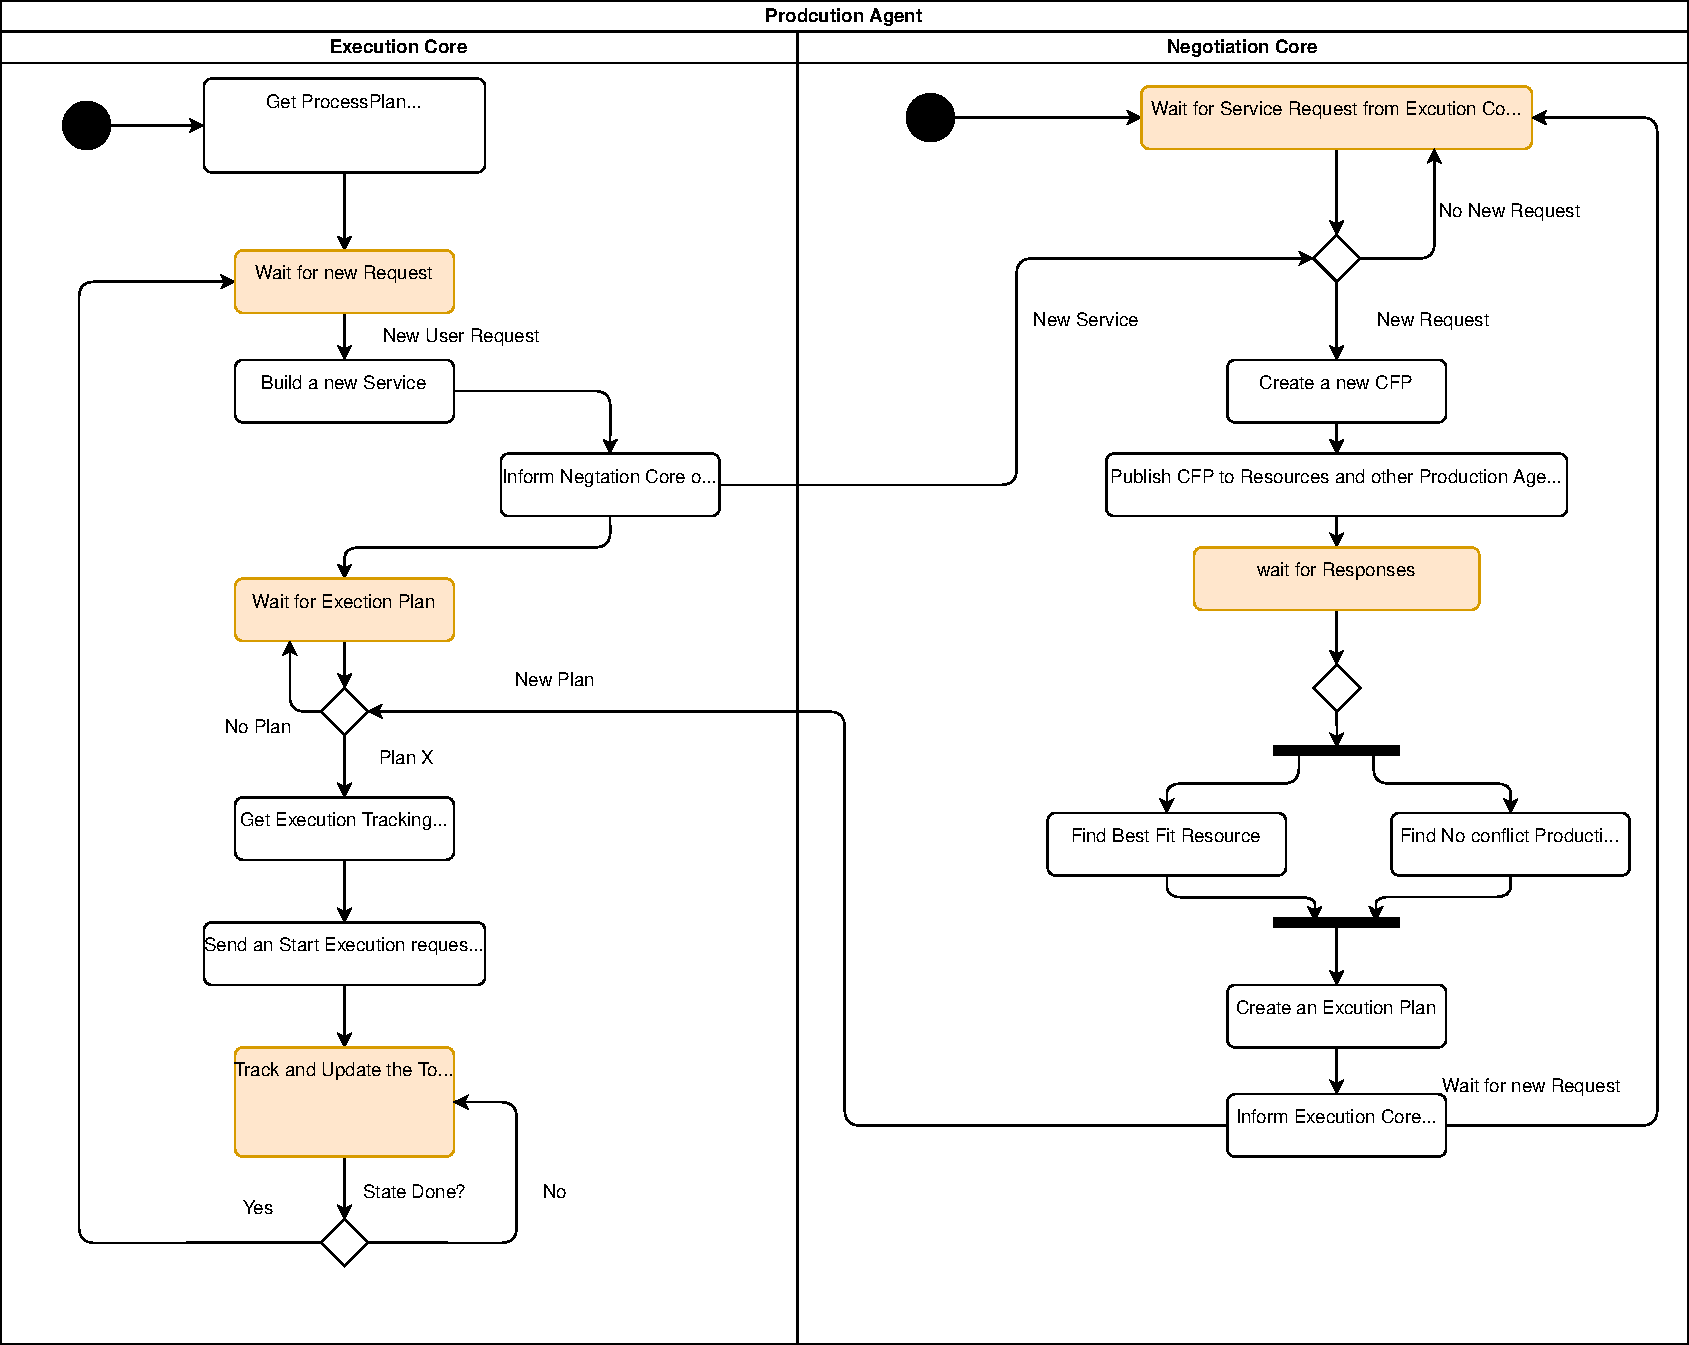
\includegraphics[width=20cm]{Images/PA_SM.pdf}
    \caption{Production Agent - Resource Agent - System Interaction State Machine}
    \label{fig:system_interaction}
\end{figure}
\end{landscape}

\subsection{Execution Core Flow}

The Execution Core operates as the entry point for production requests and manages the overall execution lifecycle:

\textbf{Request Reception.} The flow begins when a user request arrives via the \texttt{pa\_user\_service\_request} topic. The Execution Core receives and parses the request, extracting the required skills, time slot preferences, and input parameters.

\textbf{Service Delegation.} Upon receiving a valid request, the Execution Core publishes a service request to the \texttt{pa\_execution\_service\_topic}, delegating the negotiation task to the Negotiation Core. The Execution Core then enters a waiting state for the negotiation result.

\textbf{Execution Monitoring.} After receiving a positive negotiation result, the Execution Core monitors task execution by subscribing to tracking events from the selected Resource Agent. It updates the Execution Tracking Submodel as operations progress through the process plan.

\textbf{Completion Handling.} When the Resource Agent signals task completion via \texttt{job\_completion\_topic}, the Execution Core finalizes the production run and returns to waiting for the next user request.

\subsection{Negotiation Core Flow}

The Negotiation Core implements the Contract Net Protocol initiator role:

\textbf{CFP Broadcast.} Upon receiving a service request from the Execution Core, the Negotiation Core broadcasts a Call-For-Proposal to all Resource Agents subscribed to the \texttt{production\_negotiation} topic.

\textbf{Response Collection.} The Negotiation Core waits for responses from all subscribed Resource Agents. Each response is stored in a tracking dictionary, and the core checks whether all expected responses have been received.

\textbf{Parallel Response Handling.} Resource Agents respond independently and potentially in parallel. The state machine shows two parallel response paths converging at a synchronization bar, representing the collection of multiple proposals.

\textbf{Resource Selection.} Once all responses are collected, the Negotiation Core applies the best-fit selection algorithm:
\begin{enumerate}
    \item Filter responses without violations (valid proposals)
    \item Evaluate remaining proposals based on selection criteria
    \item Select the optimal resource for task execution
\end{enumerate}

\textbf{Execution Plan Creation.} After selecting a resource, the Negotiation Core creates an execution plan containing the selected resource identifier, allocated time slot, and task parameters.

\textbf{Result Publication.} The Negotiation Core informs the Execution Core of the selection result via \texttt{pa\_negotation\_result} and returns to waiting for the next negotiation request.

\subsection{Inter-Core Communication}

The two cores communicate through \ac{XMPP} publish-subscribe topics, maintaining loose coupling:

\begin{table}[ht]
\centering
\caption{Production Agent Internal Communication Topics}
\label{tab:internal_topics}
\begin{tabular}{lll}
\toprule
\rowcolor{headerblue}
\textcolor{white}{Topic} & \textcolor{white}{Publisher} & \textcolor{white}{Subscriber} \\
\midrule
pa\_execution\_service\_topic & Execution Core & Negotiation Core \\
pa\_negotation\_result & Negotiation Core & Execution Core \\
\bottomrule
\end{tabular}
\end{table}
\subsection{Resource Agent Interaction}

The Production Agent interacts with Resource Agents through external \ac{XMPP} topics:

\begin{table}[ht]
\centering
\caption{Production-Resource Communication Topics}
\label{tab:external_topics}
\begin{tabular}{lll}
\toprule
\rowcolor{headerblue}
\textcolor{white}{Topic} & \textcolor{white}{Direction} & \textcolor{white}{Purpose} \\
\midrule
production\_negotiation & PA → RA & CFP broadcast \\
negotiation\_message\_topic & RA → PA & Proposal responses \\
execution\_tracking\_topic & RA → PA & Progress updates \\
job\_completion\_topic & RA → PA & Task completion \\
\bottomrule
\end{tabular}
\end{table}
This event-driven architecture enables asynchronous coordination between the Production Agent and multiple Resource Agents, supporting scalable multi-resource scenarios without tight coupling between components.

%%%%%%%%%%%%%%%
\section{Submodel Design Considerations}

\label{sec:submodel_design}

This section addresses design decisions and scope limitations of the proposed submodel structures. It differentiates between generic (reusable) and scenario-specific elements, discusses current limitations, and provides guidance for extending the system.
\subsection{Generic vs. Scenario-Specific Elements}
\label{subsec:generic_vs_specific}

The submodel structures are designed with separation between reusable patterns and scenario-specific content. Table~\ref{tab:generic_specific} identifies which elements are transferable to other domains.

\begin{table}[ht]
\centering
\caption{Generic vs. Scenario-Specific Submodel Elements}
\label{tab:generic_specific}
\begin{tabular}{p{0.22\textwidth}p{0.35\textwidth}p{0.33\textwidth}}
\toprule
\rowcolor{headerblue}
\textcolor{white}{Submodel} & \textcolor{white}{Generic (Reusable)} & \textcolor{white}{Scenario-Specific} \\
\midrule
Operational State & Current\_State, Free\_Slots, Booked\_Slots structure & -- \\
\rowcolor{lightgray}
Knowledge & Constraints collection pattern, Constraint\_Type structure & Max\_Depth, Min\_Depth (drilling) \\
Capability & Operation with invocationDelegation, Supported\_Skills list & Drill\_Capability, MoveXY\_Capability \\
\rowcolor{lightgray}
Interaction & Time\_Slots structure, XMPP\_Endpoint & Specific time slot values \\
Process Plan & Nodes, Edges, Entry/Exit\_Point, Required\_Capabilities & Move\_Node, Drill\_Node \\
\rowcolor{lightgray}
Execution Tracking & Current\_Node, Token\_Position, Step\_Status & -- \\
\bottomrule
\end{tabular}
\end{table}
\textbf{Integrating New Resources.} To add a new resource with different capabilities (e.g., a welding machine), the following steps are required:

\begin{enumerate}
    \item \textbf{Define Capability Operations}: Create new \texttt{Operation} elements (e.g., \texttt{Welding\_Capability}) with appropriate input/output parameters and \texttt{invocationDelegation} endpoints.
    
    \item \textbf{Implement Skill Invoker}: Create a simulator or hardware interface that responds to the delegated operation calls.
    
    \item \textbf{Configure Knowledge Constraints}: Define resource-specific constraints (e.g., \texttt{Max\_Weld\_Length}, \texttt{Supported\_Materials}).
    
    \item \textbf{Register Capability String}: Add the capability identifier to \texttt{Supported\_Skills} using the same naming convention.
    
    \item \textbf{Create AgentSpeak Plans}: Add plans for the new skill execution (e.g., \texttt{+excute\_skills(welding\_capability)}).
\end{enumerate}

The submodel \textit{structure} remains unchanged; only the \textit{content} is adapted.
\subsection{Capability Matching Mechanism}
\label{subsec:capability_matching}

The current implementation uses \textbf{string-based capability matching}. The Process Plan specifies required capabilities as strings (e.g., \texttt{"Drill\_Capability"}), and Resource Agents advertise their capabilities in the \texttt{Supported\_Skills} property. During negotiation, string comparison determines compatibility.

\textbf{Limitation}: This approach is susceptible to errors:
\begin{itemize}
    \item Typographical errors (e.g., \texttt{"Drill\_Capbility"} vs. \texttt{"Drill\_Capability"})
    \item Inconsistent naming conventions across resources
    \item No semantic understanding of capability equivalence
\end{itemize}

\textbf{Recommended Extension}: Future implementations should adopt a formal capability ontology or taxonomy. Options include:
\begin{itemize}
    \item \textbf{ECLASS}: Standardized classification for products and services
    \item \textbf{IEC CDD}: Common Data Dictionary for industrial terminology
    \item \textbf{Custom OWL Ontology}: Domain-specific capability definitions with semantic reasoning
\end{itemize}

Using semantic identifiers (IRIs) instead of plain strings would enable:
\begin{itemize}
    \item Capability subsumption (e.g., \texttt{HighSpeedDrilling} is-a \texttt{Drilling})
    \item Equivalence detection across different naming conventions
    \item Automated validation of process plan feasibility
\end{itemize}
\subsection{Process Plan Structure and Limitations}
\label{subsec:process_plan_limitations}

\subsubsection{Linear vs. Precedence Graph Execution}

The current implementation supports \textbf{linear process plans} with sequential node execution. The Process Plan Submodel stores nodes and edges, but the execution logic processes nodes in a fixed sequence (Entry\_Point $\rightarrow$ ... $\rightarrow$ Exit\_Point).

\begin{figure}[ht]
\centering
\begin{tikzpicture}[node distance=2.5cm, auto,
    node/.style={circle, draw, minimum size=1cm}]
    \node[node] (A) {Move};
    \node[node, right of=A] (B) {Drill};
    \draw[->] (A) -- (B);
    \node[below=0.3cm of A, font=\scriptsize] {Entry};
    \node[below=0.3cm of B, font=\scriptsize] {Exit};
\end{tikzpicture}
\caption{Current Implementation: Linear Process Plan}
\label{fig:linear_plan}
\end{figure}

\textbf{Limitation}: True precedence graphs with parallel branches are \textbf{not supported} in the current prototype:

\begin{figure}[ht]
\centering
\begin{tikzpicture}[node distance=2cm, auto,
    node/.style={circle, draw, minimum size=0.8cm, font=\scriptsize}]
    \node[node] (A) {A};
    \node[node, above right of=A] (B) {B};
    \node[node, below right of=A] (C) {C};
    \node[node, below right of=B] (D) {D};
    \draw[->] (A) -- (B);
    \draw[->] (A) -- (C);
    \draw[->] (B) -- (D);
    \draw[->] (C) -- (D);
    \node[right=0.3cm of D, font=\scriptsize, text=red] {Not Supported};
\end{tikzpicture}
\caption{Precedence Graph with Parallel Branches (Not Implemented)}
\label{fig:precedence_graph}
\end{figure}

Extending to full precedence graph support would require:
\begin{itemize}
    \item Multiple token positions (see Section~\ref{subsec:token_position})
    \item Fork/join synchronization logic
    \item Parallel resource allocation and negotiation
\end{itemize}
\subsubsection{Capability-Node Association}

In the current design, \texttt{Required\_Capabilities} is a property at the \textbf{Process Plan level}, not associated with individual nodes:

\begin{lstlisting}[language=Python]
sm_required_capabilities = model.Property(
    id_short="Required_Capabilities",
    value="[Drill_Capability, MoveXY_Capability]"  # Plan-level
)
\end{lstlisting}

\textbf{Limitation}: This does not explicitly link which capability is needed for which node. The association is implicit through naming conventions (\texttt{Move\_Node} $\leftrightarrow$ \texttt{MoveXY\_Capability}).

\textbf{Recommended Extension}: Each node should explicitly reference its required capability:

\begin{lstlisting}[language=Python]
sm_move_node = model.SubmodelElementCollection(
    id_short="Move_Node",
    value=[
        model.Property(id_short="Required_Capability", 
                       value="MoveXY_Capability"),
        model.Property(id_short="Sequence_Number", value="1"),
        ...
    ]
)
\end{lstlisting}
\subsection{Token Position and Execution State}
\label{subsec:token_position}

The Execution Tracking Submodel uses a \textbf{single} \texttt{Token\_Position} and \texttt{Current\_Node} property:

\begin{lstlisting}[language=Python]
model.Property(id_short="Token_Position", value="1")
model.Property(id_short="Current_Node", value="Move_Node")
\end{lstlisting}

\textbf{Design Decision}: This models a single execution thread, analogous to a Petri net with one token.

\textbf{Limitation}: In a full Petri net or precedence graph, multiple tokens can exist simultaneously (parallel execution). The current design cannot represent:
\begin{itemize}
    \item Concurrent operations on different resources
    \item Fork states where execution splits
    \item Join states requiring synchronization
\end{itemize}

\textbf{Justification}: For the proof-of-concept with linear plans, a single token is sufficient. Extending to multiple tokens would require refactoring \texttt{Token\_Position} into a collection of token objects.
\subsection{Knowledge Submodel Simplifications}
\label{subsec:knowledge_limitations}

The Knowledge Submodel stores constraints as simple min/max value pairs:

\begin{lstlisting}[language=Python]
model.Property(id_short="Max_Depth", value="100.0")
model.Property(id_short="Min_Depth", value="1.0")
model.Property(id_short="Constraints_Type", value="[Max_Depth, Min_Depth]")
\end{lstlisting}

\textbf{Limitation}: This cannot express \textbf{functional dependencies} between parameters. For example:
\begin{itemize}
    \item A crane's maximum load depends on the boom extension
    \item Drilling speed limits depend on material hardness
    \item Tool wear affects achievable tolerances over time
\end{itemize}

\textbf{Recommended Extension}: Complex constraints could be modeled as:
\begin{itemize}
    \item Mathematical expressions (e.g., \texttt{MaxLoad = f(BoomLength)})
    \item Lookup tables stored as \texttt{SubmodelElementCollection}
    \item References to external constraint models (e.g., FMU/FMI)
\end{itemize}
\subsection{Assembly Processes and Bill of Materials}
\label{subsec:assembly_bom}

The current submodels include a \texttt{Preconditions} property with value \texttt{"Material Available"}, but \textbf{do not model explicit Bill of Materials (BOM)} structures.

\textbf{Scope Limitation}: The proof-of-concept focuses on machining operations (drilling, positioning) where a single workpiece is processed. Assembly scenarios with:
\begin{itemize}
    \item Multiple input parts per operation
    \item Part tracking through production stages
    \item Component-product relationships
\end{itemize}
are \textbf{not covered} by the current submodel design.

\textbf{Extension Approach}: Supporting assembly would require:
\begin{itemize}
    \item BOM Submodel with part references
    \item Material tracking in Operational State
    \item Precondition evaluation logic checking part availability
\end{itemize}
\subsection{User Request Definition}
\label{subsec:user_request}

A \textbf{User Request} is a production order submitted to the Production Agent. In the implementation, it is a message containing:

\begin{table}[ht]
\centering
\caption{User Request Message Structure}
\label{tab:user_request}
\begin{tabular}{lll}
\toprule
\rowcolor{headerblue}
\textcolor{white}{Field} & \textcolor{white}{Type} & \textcolor{white}{Description} \\
\midrule
\texttt{skills\_required} & String & Capability needed (e.g., \texttt{"drill\_capability"}) \\
\texttt{at\_time} & String & Requested time slot (e.g., \texttt{"10:30-11:00"}) \\
\texttt{input\_arguments} & Dictionary & Operation parameters (X, Y, Depth, RPM) \\
\bottomrule
\end{tabular}
\end{table}

The User Request is published to the \texttt{pa\_user\_service\_request} XMPP topic and received by the Execution Core, which initiates the negotiation process.
\subsection{Concrete Example: Drill Operation}
\label{subsec:concrete_example}

To illustrate how the submodels work together, consider a complete drill operation request:

\textbf{Step 1: User Request}
\begin{lstlisting}
{
  "skills_required": "drill_capability",
  "at_time": "10:30-11:00",
  "input_arguments": {"X": 60, "Y": 50, "Depth": 5, "RPM": 1500}
}
\end{lstlisting}

\textbf{Step 2: Process Plan Lookup}

The Production Agent reads the Process Plan Submodel:
\begin{itemize}
    \item \texttt{Entry\_Point}: \texttt{"Move\_Node"}
    \item \texttt{Exit\_Point}: \texttt{"Drill\_Node"}
    \item \texttt{Edges}: \texttt{"Move\_Node to Drill\_Node"}
    \item \texttt{Required\_Capabilities}: \texttt{"[Drill\_Capability, MoveXY\_Capability]"}
\end{itemize}

\textbf{Step 3: Resource Discovery}

The Negotiation Core broadcasts a CFP. Resource Agent 1 checks its Capability Submodel:
\begin{itemize}
    \item \texttt{Supported\_Skills}: \texttt{"drill\_capability, movexy\_capability"} \checkmark
\end{itemize}

And its Interaction Submodel:
\begin{itemize}
    \item \texttt{Free\_Slots}: includes \texttt{"10:30-11:00"} \checkmark
\end{itemize}

And its Knowledge Submodel:
\begin{itemize}
    \item \texttt{Max\_Depth}: 100mm $\geq$ requested 5mm \checkmark
\end{itemize}

\textbf{Step 4: Execution}

After selection, the Resource Agent executes:
\begin{enumerate}
    \item Invoke \texttt{MoveXY\_Capability} with X=60, Y=50
    \item Update \texttt{Current\_Node} = \texttt{"Move\_Node"}, \texttt{Step\_Status} = \texttt{"running"}
    \item On completion: \texttt{Step\_Status} = \texttt{"completed"}
    \item Invoke \texttt{Drill\_Capability} with Depth=5, RPM=1500
    \item Update \texttt{Current\_Node} = \texttt{"Drill\_Node"}, \texttt{Step\_Status} = \texttt{"running"}
    \item On completion: \texttt{Step\_Status} = \texttt{"completed"}
\end{enumerate}

\textbf{Step 5: Completion}

The Execution Tracking Submodel final state:
\begin{itemize}
    \item \texttt{Token\_Position}: 2 (at Exit\_Point)
    \item \texttt{Current\_Node}: \texttt{"Drill\_Node"}
    \item \texttt{Step\_Status}: \texttt{"completed"}
\end{itemize}

This example demonstrates how the generic submodel structures are populated with scenario-specific content to execute a concrete production task.
